\documentclass[12pt,a4paper,oneside]{book}

% Packages
% Packages

% Language-related

\usepackage{setspace}
\usepackage[T1,T2A]{fontenc}
\usepackage[utf8]{inputenc}
\usepackage[english,bulgarian]{babel}

% Others
\usepackage{indentfirst}
\usepackage{amsmath}
\usepackage{blindtext} % Needed for creating dummy text passages
\usepackage[colorlinks=true,breaklinks,english]{hyperref}
\usepackage[hyphenbreaks]{breakurl}
\usepackage{xcolor}
\usepackage{ragged2e}
\definecolor{c1}{rgb}{0,0,0} % Blue
\definecolor{c2}{rgb}{0,0.3,0.9} % Light blue
\definecolor{c3}{rgb}{0.3,0,0.9} % Red blue
\hypersetup{
    linkcolor={c1}, % Internal links
    citecolor={c2}, % Citations
    urlcolor={c3} % External links/URLs
}

%\usepackage{cite} % Needed for cite

% Needed for cite and abbrvnat bibliography style
\usepackage[round,authoryear]{natbib}

% Needed for displaying bibliography and other in the table of contents
\usepackage[nottoc]{tocbibind}

\usepackage{graphicx} % Needed for \includegraphics
\usepackage{epstopdf}
\usepackage{longtable} % Needed for long tables over pages
\usepackage{bigstrut} % Needed for the command \bigstrut
\usepackage{enumerate} % Needed for some options in enumerate
\usepackage{todonotes} % Needed for todos
\usepackage{makeidx} % Needed for creating an index
\makeindex


% Page settings
% Page settings

% Needed for page border settings
\usepackage[top=1.8cm, bottom=1.8cm,left=2.0cm,right=2.0cm]{geometry}

% For writing with hyphenless justification (tries to)
\sloppy

\hyphenation{}
\hyphenpenalty=10000
\exhyphenpenalty=10000


% Custom commands

% This file defines some macros

% Text-bold-italic (makes the text bold and italic)
\newcommand{\tbi}[1]{\textbf{\textit{#1}}}

% Underline and italic
\newcommand{\imp}[1]{\underline{\textit{#1}}}


\begin{document}

\pagestyle{empty}
\begin{titlepage}

\center % Center everything on the page

\vspace{5mm}
\textsc{\Large Технологично училище Електронни системи към Технически
  университет - София}\\[0.5cm] % TUES ftw

\vspace{30mm}

{\Large \bfseries ДИПЛОМНА РАБОТА}\\[2cm]

\Large Тема: Мрежов анализатор с възможност за отдалечен анализ посредством
AngularJS 2 клиент

\vspace{40mm}

\begin{minipage}{0.35\textwidth}
\begin{flushright} \normalsize
Дипломант: \\[5mm]
Научен ръководител: \\[5mm]
\end{flushright}
\end{minipage}
~
\begin{minipage}{0.55\textwidth}
\begin{flushleft} \normalsize
Ивайло Арнаудов \\[5mm]
Стоил Стоилов\\[5mm]
\end{flushleft}
\end{minipage}\\[2cm]

{\normalsize София, $2017$} \\[0cm]


\vfill % Fill the rest of the page with whitespace

% List of symbols (kept just in case so far)

\newpage
\begin{flushleft}
\begin{Large}
\emph{\bf Списък на означения}\\
\end{Large}
\end{flushleft}
\begin{spacing}{1.241}
\vspace{10mm}
\begin{minipage}{0.2\textwidth}
\begin{flushleft} \normalsize
\ensuremath{\sigma_{y}(\tau)}\\
\end{flushleft}
\end{minipage}
~
\begin{minipage}{0.5\textwidth}
\begin{flushleft} \normalsize
Exponential regression function\\
\end{flushleft}
\end{minipage}\\[4cm]
\end{spacing}
\vfill

% List of abbreviations

\newpage
\begin{flushleft}
\begin{Large}
\emph{\bf Списък на съкращения}\\
\end{Large}
\end{flushleft}
\begin{spacing}{1.241}
\vspace{10mm}
\begin{minipage}{0.2\textwidth}
\begin{flushleft} \normalsize
VPN\\
\end{flushleft}
\end{minipage}
~
\begin{minipage}{0.5\textwidth}
\begin{flushleft} \normalsize
Virtual Private Network\\
\end{flushleft}
\end{minipage}\\[4cm]
\end{spacing}
\vfill

\pagestyle{plain}

\blankpage

\tableofcontents
\vfill
\chapter*{Увод}

\section{Компютърни мрежи}

Всеки от последните три века бива доминиран от някаква нова технология ---
механичните системи на Индустриалната революция през
XVIII век, парния двигател през XIX век и събирането, обработката и дистрибуцията
на информация през XX век. С развитието
на последната човечеството става свидетел на инсталацията на глобални мрежи,
изобретяването на радиото и телевизията, развитието на
компютърната индустрия, и създаването на Интернет. Като резултат от огромния
технологичен прогрес в сферата на информационните технологии, през XXI век
разликите между съхраняване, транспортиране и обработка на информация изтъняват,
а успоредно с това растат и изискванията на крайния потребител към
комуникационните услуги.

Въпреки крехката възраст на компютърната индустрия, тя прави значителен прогрес.
През първите две десетилетия от съществуването им, компютърните системи са били
силно централизирани.  Университет или средно голяма фирма биха имали един или
два компютъра, а по-големите институции --- по няколко. Обединяването на
компютрите и комуникациите означава, че старият модел при който един такъв
компютър изпълнява заявките на цялата организация бива заменен от нов модел, при
който голямо количество отделни, но взаимносвързани компютри, извършват обработка
на дадена информация. Системите, участващи в този модел, се наричат \textit{компютърни мрежи}.
\cite{tanenbaum_computer_2011}

\section{Приложения на компютърните мрежи}

\subsection{Приложения на компютърните мрежи в бизнесa}

Един от основните проблеми, който решават компютърните мрежи е споделянето на
ресурси --- например общ принтер. Но далеч по-важен проблем, който те решават,
е споделянето на информация. Компаниите са фундаментално зависими от дигиталната
информация. Повечето компании имат записи за клиенти, за продукти и т.н. онлайн.

Мрежите предоставят и механизми за по-богати форми на виртуална комуникация --
споделяне на екрана, видеоконференции, споделена обработка на документи.
Те отварят вратите и за нов бизнес модел, наречен \textit{електронна
търговия} (\textit{e-commerce}) \cite{tanenbaum_computer_2011}, който се
развива с големи темпове и става де факто стандарт при търговията от всякакъв тип.
\subsection{Приложения на компютърните мрежи в дома}

В началото на компютърната индустрия причините за покупка на компютър от крайния
потребител са се свеждали до нуждата от обработка на текст и игри. През XXI век
основната причина е нуждата от достъп до
Интернет. Аналогично на компаниите, крайните потребители могат да достъпват
отдалечена информация, да комуникират посредством \textit{социални мрежи},
да купуват продукти и услуги чрез \textit{e-commerce} системи, да използват електронно
банкиране, да споделят мултимедия и софтуер, да колаборират посредством
\textit{wiki} сайтове и др.

Друго напоследък развиващо се приложение на мрежите в дома е концепцията за
\textit{Internet of Things}. Основната й характеристика е, че електронните
устройства на крайните потребители се включват в компютърните мрежи. Например,
душа в банята, който традиционно не е компютър, би могъл да записва какво количество
вода е използвано и да изпраща информацията на приложение, което изчислява как
водата да бъде използвана по-ефективно.

\section{Изисквания към мрежов анализатор}

Споменатият етап на развитие на компютърните мрежи предразполага към
по-комплексни инструменти и процеси за мониторинг и отстраняване на проблеми в
мрежата. \textit{Мрежовия анализатор}
e инструмент, който помага на мрежовия администратор, предоставяйки услугата
\textit{aнализ на пакети} (\textit{packet analysis}, \textit{packet sniffing}).
Анализът на пакети описва процеса на заснемане и интерпретиране на данни в
реално време (т.е в момента на преминаване през преносвателната среда).
Изискванията към един такъв анализататор е да улесни мрежовия администратор
с изпълнението на следните задачи:

\begin{itemize}
  \item
  Идентифициране и задълбочено разбиране на процесите в мрежата
\item
  Идентифициране на участниците в мрежата, потенциални причинители на атаки или
  злонамерена активност
\item
  Изследване кой или какво използва наличния капацитет на преносвателната
  среда, както и на моментите на максимално използване (load) на мрежата
\end{itemize}

Представеното в текущата дипломна работа приложение има за цел да спази тези
изисквания като, взимайки предвид вече описаното развитие на компютърните мрежи
с оглед необходимостта от колаборация и децентрализираност, предостави на
мрежовия администратор и възможност за сигурно, отдалечено достъпване на мрежовия
анализатор, както и споделен преглед на анализа с други администратори.

\justify
\chapter{Методи и технологии за реализиране на мрежови анализатори}

\section{Основни принципи, технологии и развойни среди за реализиране на мрежови
анализатори}

\subsection{Основни принципи}
Процеса на анализ на пакети включва кооперация между софтуера и хардуера и може
да бъде разделен в следните три стъпки:

\begin{itemize}
  \item
    \textbf{Събиране} В началната фаза на работата си, анализатора събира
    'сурови', неинтерпретирани данни в двоичен вид директно от проводника.
    Типично това става като съответно избрания мрежови интерфейс за анализ
    бива превключен в т.нар.  \textit{promiscuous} режим. В този режим мрежовата
    карта може да прихваща всевъзможен трафик по дадения мрежови сегмент, а не
    просто такъв, адресиран до станцията.
  \item
    \textbf{Конвертиране} В следващата фаза на работата си, анализатора
    конвертира събраните данни в разбираем формат за крайния потребител. След тази
    стъпка, данните събрани от преносвателната среда са във вид, който може да
    бъде интерпретиран на много основно ниво; останалата по-голяма част от
    анализа се оставя на крайния потребител.
  \item
    \textbf{Анализ} В третата и финална фаза, мрежовият анализатор извършва
    реалния анализ на събраната и конвертирана информация. Анализатора взима
    събраните данни, отчита използвания мрежови протокол, базирайки се на
    извлечените до момента данни, и започва да анализира конкретните свойства на
    протокола.
\end{itemize}

С цел да бъде разбран процеса на работа, а и съответно модела на реализация на
мрежов анализатор, е необходимо дефиниране на основните принципи на
комуникация между компютърните системи.

\subsubsection{Протоколни архитектури}

За да се намали комплексността на решенията, повечето мрежи са организирани като
стек от \textit{слоеве} или \textit{нива}, всеки изграден върху слоя под него.
Броя на слоевете, имената на всеки от тях, съдържанието на всеки и функциите,
които изпълнява са различни за различните мрежи. Целта на всеки слой е да
предостави конкретни услуги на разположените по-високо от него в йерархията
слоеве като им спестява детайлите около имплементацията на тези услуги.

Тази концепция е широко популярна в компютърните науки, още известна е като
криене на имплементационни детайли, абстрактни типове от данни, енкапсулация на
данни. Фундаменталната идея е, че дадена част от софтуера (или хардуера)
осигурява услуга на потребителите си, но скрива от тях детайлите на вътрешното
си състояние и алгоритмите.

Когато слоят \textit{n} на една машина е във връзка със слоят \textit{n} на
друга машина, правилата и конвенциите използвани в тази връзка се наричат
\textit{протокол на n-ти слой}. На практика, протокол е договореност
между комуникиращите страни относно това как протичат процесите на
комуникацията между тях. \cite{tanenbaum_computer_2011} Протоколите могат да
бъдат прости или комплексни. Някои от общите
свойства, които традиционно споделят, макар и абстрактно представени
\cite{sanders_practical_2011}, са:

\begin{itemize}
  \item \textbf{Инициация на връзка} Дефинира кой инициира връзката, например
    клиентът или сървърът. При иницииране на връзка може да е необходима и
    допълнителна служебна информация преди да протече обмена на полезна
    информация.
  \item \textbf{Договаряне на параметрите на връзката} Дефинира процес, в който
    двете страни се разбират --- дали връзката е криптирана, как се пренасят
    ключовете за декриптиране, какъв тип е връзката (full/half duplex) и др.
  \item \textbf{Форматиране на данните} Дефинира подредбата на данните, в каква
    последователност се обработват от приемащата страна и др.
  \item \textbf{Откриване на грешки и корекция на грешки} Дефинира какво се
    случва при загуба на данни, как едната страна на връзката реагира при липса
    на отговор от другата и др.
  \item \textbf{Терминиране на връзка} Дефинира как дадено крайно устройство
    сигнализира на друго че връзката е приключила, каква финална информация
    трябва да бъде предадена преди успешния край на връзката и др.
\end{itemize}

Традиционно, тези протоколи не 'живеят' сами, а са основополагащи за цялостния
процес на комуникация.  Например, на \autoref{five_layer_network_fig} е
представен пет слоен модел на комуникация между двa софтуерни процеса. Реално
данни не се предават директно от слой \textit{n} на едната машина до слой
\textit{n} на другата: комуникацията е \textit{виртуална} (означена с прекъснати
линии на \autoref{five_layer_network_fig}).
Вместо това, всеки слой предава данни и контролна информация на този под него
докато не се достигне най-ниския слой. Под първия слой е физическият, т.е
преносвателната среда, през която реалната комуникация се случва. (означено с
непрекъснати линии на \autoref{five_layer_network_fig})

\begin{figure}[h!]
  \centering
  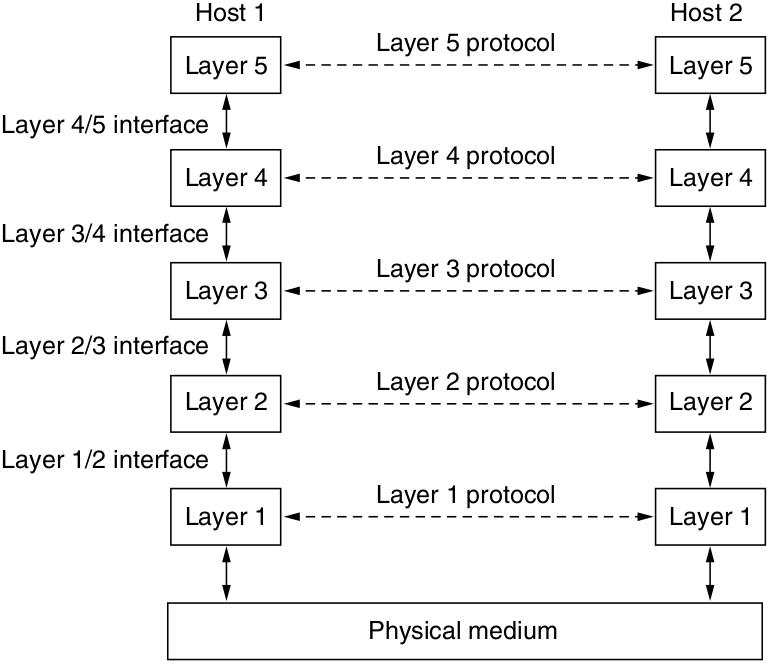
\includegraphics[width=0.6\textwidth]{figures/five_layer_network.png}
  \caption{Модел на пет слойна мрежа}
  \label{five_layer_network_fig}
\end{figure}

Между всяка съседна двойка слоеве има \textit{интерфейс}. Този интерфейс
дефинира какви операции и услуги долният слой предлага на горния. Интерфейсите
между слоевете трябва да бъдат ясно дефинирани. Това впоследствие би улеснило
замяната на един слой с напълно различен протокол или имплементация (например
смяна на телефонни линии със сателитни такива), защото единственото, което се
очаква от новия протокол, е да предлага \textit{точно} същото множество услуги
на горния слой като стария. Аналогично, този механизъм позволява един протокол
да се промени в даден слой без знанието на слоевете под и над него.

\subsubsection{Основен механизъм на междуслойна комуникация. Капсулиране и
декапсулиране.}

Основния механизъм на междуслойна комуникация е фундаментален за имплементацията
на представения в дипломната работа мрежов анализатор. Той може да бъде описан
с помощта на пет слойния модел представен във
\autoref{interlayer_communication_fig}.
В случая, даден процес иска да изпрати съобщението \textit{M}. От петия
слой, съобщението бива предадено на четвъртия слой за изпращане. Четвъртият
слой слага \textit{заглавна част} (\textit{header}) в началото на съобщението и предава резултата
към трети слой. Заглавната част включва служебна информация, например адреси, за да
може съответния четвърти слой на приемната машина да достави съобщението. Други
примери за служебна информация могат да бъдат \textit{числови поредици}
(\textit{sequence numbers}) --- често използвани когато слоят на по-ниско ниво
няма функционалност за запазване на последователността на съобщенията,
както и размери и времена.

\begin{figure}[h!]
  \centering
  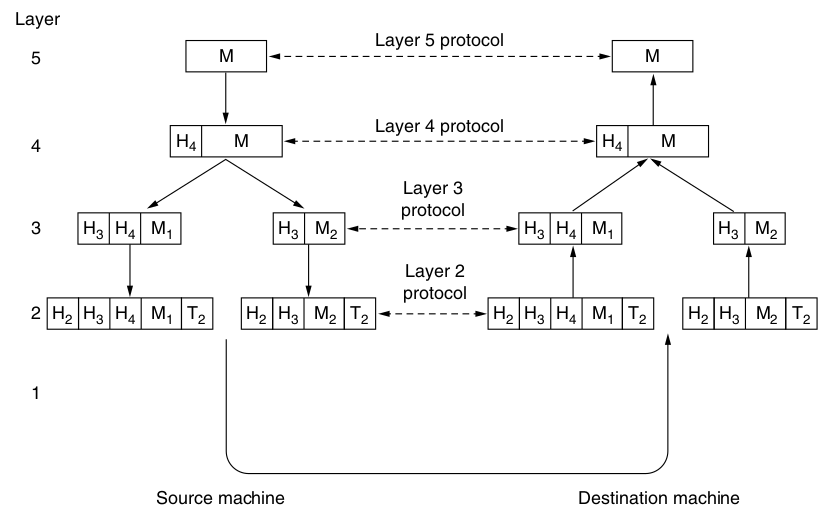
\includegraphics[width=0.8\textwidth]{figures/interlayer_communication.png}
  \caption{Междуслойна комуникация. Капсулиране и декапсулиране.}
  \label{interlayer_communication_fig}
\end{figure}

В много мрежи, често няма граница относно размера на съобщения на четвърти слой,
но почти винаги има такава относно размера от самия протокол на трети слой.
Следователно, третият слой трябва да раздели идващите съобщения на по-малки
единици --- пакети, като успоредно с това добавя заглавна част към всеки пакет. В
случая на \autoref{interlayer_communication_fig}, съобщението \textit{M} се
разделя на две части: \textit{M\textunderscript{1}} и
\textit{М\textunderscript{2}}.

Третият слой аналогично предава пакетите на втория слой, който от своя страна
освен че добавя заглавна част, добавя и крайна част (\textit{'ремарке'}, \textit{trailer}). Резултата
се предава на първия слой, който се занимава с физическия пренос на данните.
Описаният процес е още известен като \textit{капсулация} (\textit{encapsulation}). В
приемащата страна, съобщението се \textit{декапсулира} (\textit{decapsulation}) като
всяка заглавна част се отделя успоредно с 'изкачването' на съобщението нагоре по
слоевете. Нито една заглавна част за слоевете под \textit{n}-тия не достига до
\textit{n}-ти слой. Едновременно с това, на
\autoref{interlayer_communication_fig} ясно проличават виртуалната и реална
комуникация, както и разликите между протоколи и интерфейси. Например, на
четвърти слой процесите концептуално интерпретират комуникацията си като
хоризонтална, използвайки протокола на четвърти слой, и биха имали функции от типа
на \texttt{send()} и \texttt{recieve()}, макар че в действителност те
комуникират с по-ниските слоеве през 3/4 интерфейса.

\subsubsection{Имплементации на протоколни архитектури}

\paragraph{Open Systems Interconnection (OSI)} представлява модел на свързване
на отворени системи, т.е системи отворени за комуникация с други такива.
Развит от Международната организация по стандартизация (ISO), той
има седем слоя:

\begin{itemize}
  \item \textbf{Physical} Физическият слой се занимава с предаването на битове
    информация в чист вид посредством електрически сигнали.
  \item \textbf{Data Link} Каналният слой се занимава с контрола на достъпа до
    споделената преносвателна среда и създаването на абстракция върху
    чистия пренос на данните. Това става чрез разделянето на
    изпращаните данни в единица, наречена \textit{кадър} (\textit{frame}) и изпращането й
    последователно.
  \item \textbf{Network} Мрежовият слой се занимава с маршрутизацията на
    пакети от подател към получател.
  \item \textbf{Transport} Транспортният слой се занимава с разделянето на
    получените данни от слоевете над него, подаването им към
    мрежовия слой и гарантиране на успешния им пренос.
  \item \textbf{Session} Сесийният слой се занимава с установяването на
    \textit{сесии} между потребителите на две машини. Примерни услуги са контрол
    на диалога и синхронизация.
  \item \textbf{Presentation} Представителният слой се занимава с синтаксиса и
    семантиката на изпратената информация.
  \item \textbf{Application} Приложеният слой се занимава с преноса на данни на
    ниво приложения, типични представители за такива протоколи са HTTP, FTP и
    т.н.
\end{itemize}


\paragraph{TCP/IP} представлява първият модел на работа на
компютърните мрежи, разработен първоначално през 1974г. за да опише
функционалността на ARPANET. OSI моделът на практика представлява негово
разширение. TCP/IP моделът е съставен от 4 слоя:

\begin{itemize}
  \item \textbf{Link} Каналният слой описва какви връзки да бъдат използвани,
    например серийни или класически Ethernet, като по-скоро представлява не
    слой, а интерфейс между преносвателната среда и машините.
  \item \textbf{Internet} Мрежовият слой се занимава с маршрутизацията на
    пакети от подател към получател. Класически примери за протоколи, опериращи
    на слоя са IP и ICMP.
  \item \textbf{Transport} Транспортният слой се занимава с разделянето на
    получените данни от слоевете над него, подаването им към
    мрежовия слой и гарантиране на успешния им пренос. В зависимост от нуждата
    за надеждност на преноса има два типични протокола: TCP и UDP.
  \item \textbf{Application} Приложеният слой се занимава с преноса на данни на
    ниво приложения, типични представители за такива протоколи са HTTP, FTP и
    т.н.
\end{itemize}

\begin{figure}[h!]
  \centering
  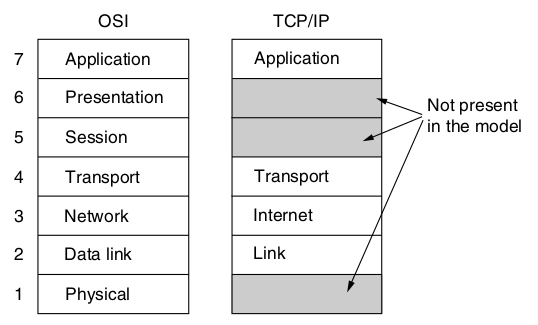
\includegraphics[width=0.7\textwidth]{figures/osi_vs_tcp.png}
  \caption{Сравнение между OSI и TCP/IP}
  \label{osi_vs_tcp_Fig}
\end{figure}

\paragraph{Основен принцип за прихващане на данни от преносвателната среда}

Обикновено когато мрежовата карта получи кадър, тя проверява дали адресът на
получателя съвпада с нейния собствен. Ако съвпада, тя генерира прекъсване към
процесора. Функцията, обработваща прекъсването, е драйвeрът за мрежовата
карта в ядрото на операционната система. Драйверът 'закача' \textit{времева
щампа}
(\textit{timestamp}) върху приетите данни и копира данните от буфера на картата
в заделен блок от памет в ядрото на операционната система. След това системния
протоколен стек обработва данните чрез процеса на декапсулация и ги предава към
потребителското приложение.

При типичната имплементация на мрежов анализатор, пакетите следват аналогичен
път, но с малка промяна: драйверът копира приети или изпратени данни в част от
ядрото на операционната система наречено \textit{пакетен филтър}
(\textit{packet filter}). По подразбиране,
пакетните филтри пропускат всеки пакет, но поддържат комплексни филтри.
Важно е да се отбележи, че в следствие от местоположението си, пакетните филтри
изискват административни привилегии, тъй като копирането на получени или изпратени
пакети предполага риск за сигурността. На \autoref{bpf_overview_fig} е
илюстриран описаният процес с помощта на Berkley пакетния филтър (BPF),
механизъм, стоящ в основата на libpcap.

\begin{figure}[h!]
  \centering
  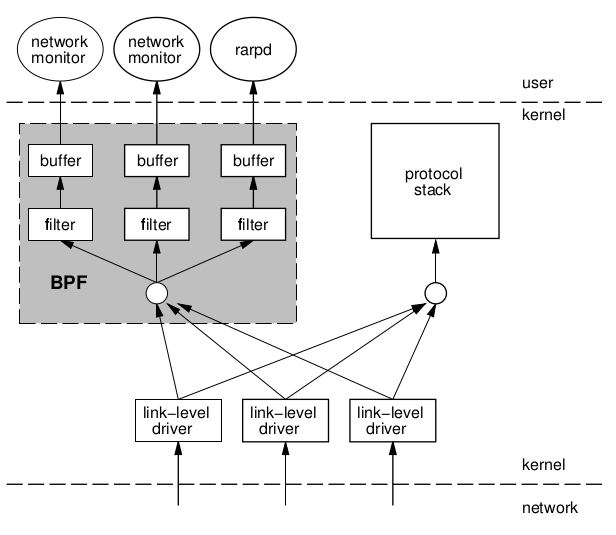
\includegraphics[width=0.7\textwidth]{figures/bpf_overview.png}
  \caption{Преглед на имплементацията на мрежов анализатор на ниво ядро на
  операционната система}
  \label{bpf_overview_fig}
\end{figure}

\subsection{Основни технологии}

\subsubsection{libpcap}

\textbf{libpcap} е библиотека с отворен код, която осигурява интерфейс на високо
ниво за системи за прихващане на пакети от преносвателната среда. Създадена е
през 1994г. от Ван Якобсен, Крейг Леърс и Стивън МакКейн, изследователи в
Lawrence Berkeley National Laboratory към University of California,
като част от научен проект за изследване и подобрение на TCP. Интерфейсът на
libpcap е основно достъпен на програмните езици C и C\texttt{++}.
Същестуват и голямо количество библиотеки
енкапсулиращи функционалността й на езици като Perl, Python, Java, C# или Ruby.

\subsubsection{WebSocket}

\textbf{WebSocket} представлява комуникационен протокол, позволяващ двустранна
(full-duplex) връзка в реално време между клиент и сървър върху TCP. Типичното му
приложение е в уеб браузърите и уеб сървърите (тъй като при началното ръкостискане се използва
HTTP \texttt{Upgrade} заявката), но на практика може да се приложи от всеки тип
клиент-сървър приложение. Протокола е стандартизиран през 2011г. в RFC 6455.

\subsubsection{Angular 2}

\textbf{Angular 2} представлява framework за разбработка на едностранични
(SPA) уеб приложения. Наследникът на AngularJS имплементира компонентно-базирана
архитектура чрез Web Components спецификацията, което предразполага към вградена
поддръжка от браузъра, по-добра енкапсулация и по-голяма ефективност. Подобно на
предшественика си, Angular 2 залага на тестваемостта и модулярността, като освен
разширена функционалност за инжектиране на зависимости (dependency injection),
за да улесни още повече разработката на големи приложения,
акцентира върху еднопосочеността на данните (unidirectional data flow) и
използването на статично типизиран език --- TypeScript, който представлява
надграждане (superset) на ECMAScript 2016 стандарта.

\subsection{Основни развойни среди}

\subsubsection{Eclipse CDT}

\textbf{Eclipse CDT} предоставя напълно функционална развойна среда за програмиране на
езиците C и C++, базирана на платформата Eclipse. По-забележителните
характеристики са: поддръжка на множество системи за автоматизиране на процеса
на компилация, навигация на изходния код, йерархия на типовете, граф на
извикванията, навигация на макроси, рефакториране и генерация на програмен код,
инструменти за дебъгване, включително такива за преглед на паметта, регистрите и
деасемблиране.

\subsubsection{Qt Creator}

\textbf{Qt Creator} e мултиплатформена среда среда за разработка, част от
SDK на популярния framework за разработка на графични
интерфейси Qt. Някои от забележителните характеристики на средата са: поддръжка
на визуално дебъгване на програмния код, интерактивен дизайнер на подредбата на
графичния интерфейс, поддръжка на множество системи за автоматизация на процеса
на компилация, поддръжка на множество системи за контрол на изходния код (VCS),
поддръжка на инструменти за симулация на приложението за мобилни устройства.
Разбира се, средата е предимно подходяща за разработка, когато се използва Qt.

\section{Съществуващи решения и реализации}

Преди да се разгледат същестуващите решения и реализации е важно да се споменат
критериите, необходими за оценяване на полезността на един мрежов анализатор:

\begin{itemize}
  \item \textbf{Поддържани протоколи} Всички мрежови анализатори могат да
    интерпретират множество от протоколи. Повечето могат да интерпретират
    най-основните протоколи от мрежовия слой -- например IPv4 и ICMP; от
    транспортния слой -- TCP и UDP, както и от приложения -- DNS и HTTP.
    Не всички обаче поддържат нетрадиционни или нови протоколи (например IPv6).
  \item \textbf{Потребителски интерфейс} От значение е цялостния изглед на
    приложението, колко лесно се инсталира, колко лесно се извършват
    необходимите операции посредством интерфейса. От значение е и опита на
    анализиращия -- типично, по-опитният анализиращ би предпочел анализатор
    използващ командния ред, начинаещият -- анализатор с графичен интерфейс.
  \item \textbf{Цена} Голямо количество от мрежовите анализатори са
    свободно-използваеми и конкуриращи се с платени такива. Обикновенно
    разликата между платените и свободно-използваемите е при прегледа на
    анализа, който е по-пълноценнен при платените.
  \item \textbf{Програмна поддръжка} Обикновенно при изникването на проблем
    анализиращият трябва да има солидна база от източници на решения --
    документация на анализатора, публични форуми, блогове и т.н. Фундаментално
    при избора на анализатор е до колко са налични тези източници.
  \item \textbf{Поддръжка на операционната система} Не всеки анализатор поддържа
    всяка операционна система. Основополагащо за избора на анализатор е
    операционната система под която се очаква той да функционира.
\end{itemize}


\subsection{Wireshark}

Wireshark има дълга история. Програмата е оригинално създадена от Джералд Комбс,
студент по комютърни науки. Първата версия на приложението на Комбс се нарича
Ethereal и за първи път е пуснато през 1998г. под GPL. Осем
години след пускането на Ethereal, той напуска работа, но за съжаление
неговият работодател има пълни права върху името Ethereal. Така през средата на
2006г. се ражда Wireshark.

Wireshark предлага няколко предимства които я правят подходяща за всекидневна
употреба. Програмата таргетира както по-напредналите с мрежовия анализ, така и
начинаещи.

\begin{itemize}
  \item \textbf{Поддържани протоколи} Поддържа над 850 различни протокола --- от
    по-популярните като IP и DHCP, до по-комплексни частни протоколи като
    AppleTalk и BitTorrent. Вземайки предвид факта че Wireshark се разработва на
    принципа на отворения код, нов протокол се добавя с всяка нова версия. В
    случай че необходим на анализиращия протокол не е имплементиран, той може да
    бъде имплементиран като разширение и изпратен до разработчиците на
    Wireshark.
  \item \textbf{Потребителски интерфейс} Един от най-лесните за употреба
    потребителски интерфейси. Типичен GUI с ясно
    описани контекстни менюта и интуитивно оформление. Поддържа цветово кодиране
    спрямо протокола както и детайлен преглед на неинтерпретираните данни. За
    разлика от tcpdump, Wireshark GUI е идеална за начинаещия в мрежовия анализ.
    Разделен е на три компонента: Packet List (списък от пакети),
    Packet Details (детайли за избрания пакет), Packet Bytes (преглед на пакета
    в неинтерпретиран вид). Цялостен изглед на интерфейса може да бъде видян на
    \autoref{wireshark_fig}.
  \item \textbf{Цена} Тъй като програмата се разработва на принципа на отворения
    код, тя е изцяло безплатна и може да се използва според GPL лиценза.
  \item \textbf{Програмна поддръжка} Тъй като програмата се разработва на
    принципа на отворения код, тя няма формална поддръжка --- тя се
    базира на обществото от потребители на програмата. Уеб страницата на
    Wireshark има връзки към няколко форми за поддръжка: онлайн документация,
    wiki за разработчици, FAQ, както и връзки към официалната мейл листа.
  \item \textbf{Поддръжка на операционната система} Поддържа всички модерни
    операционни системи: Microsoft Windows, Mac OS X и Linux базираните
    операционни системи.
\end{itemize}

\begin{figure}[h!]
  \centering
  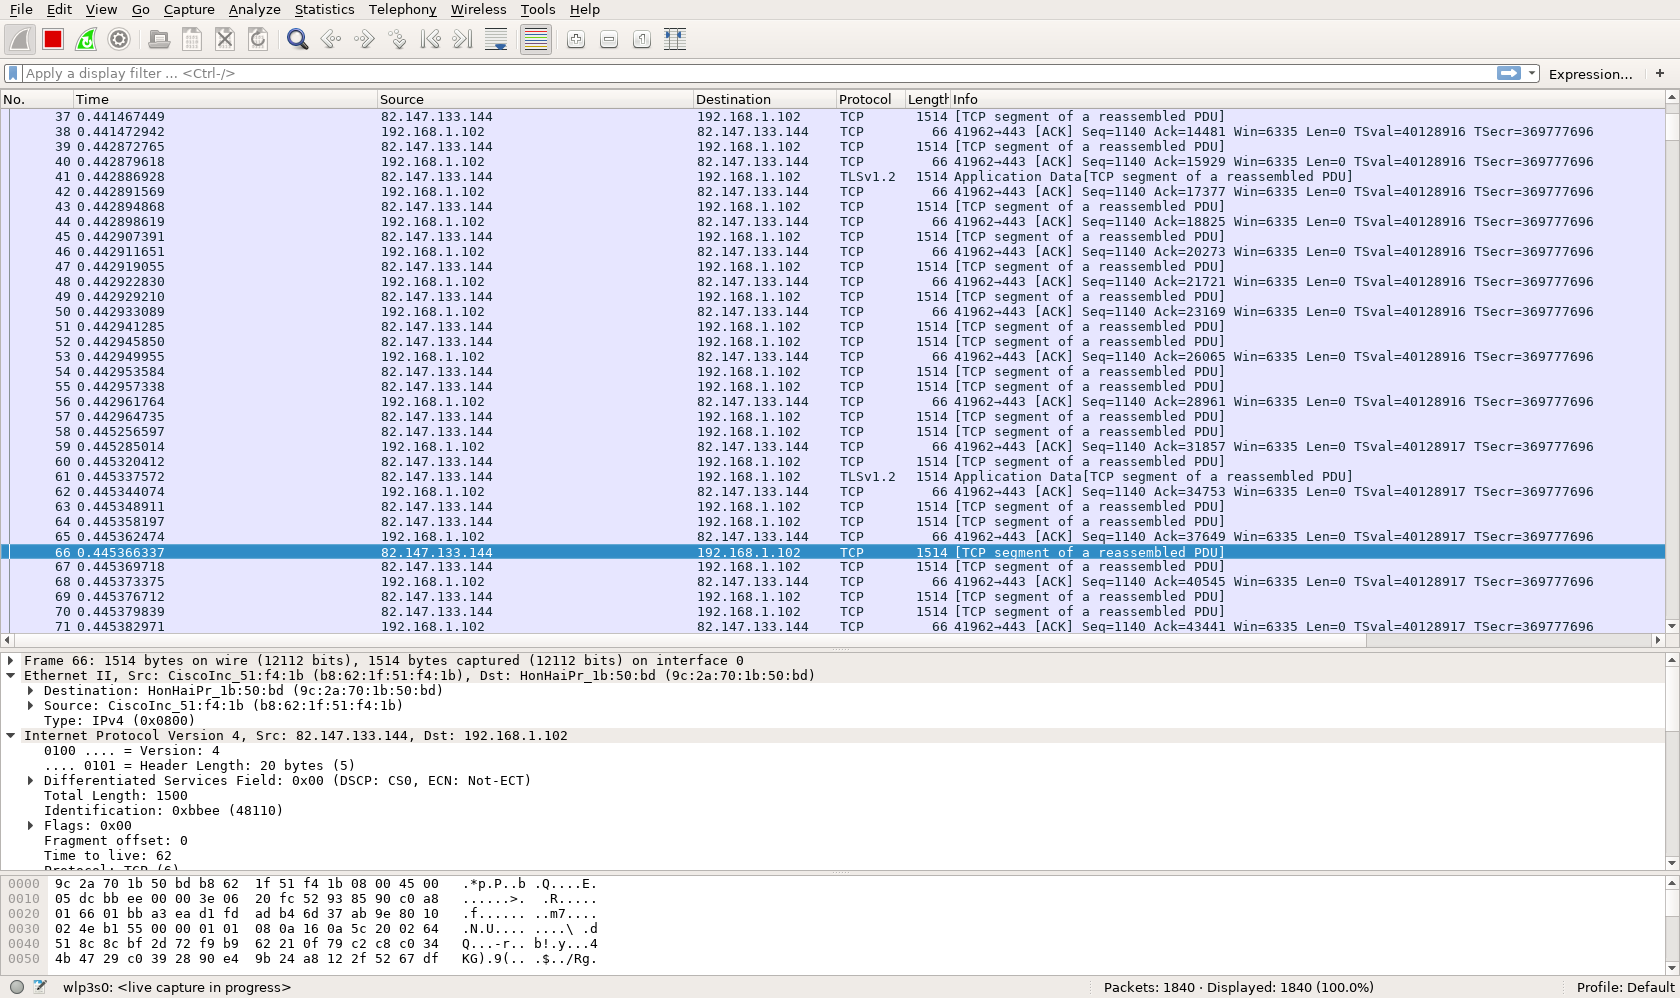
\includegraphics[width=1.0\textwidth]{figures/wireshark.png}
  \caption{Изглед на потребителския интерфейс на Wireshark.}
  \label{wireshark_fig}
\end{figure}

\subsection{tcpdump}

Първата версия на програмата е написана през 1987г. от Ван Якобсен,
Крейг Леърс и Стивън МакКейн, няколко години преди написването на libpcap.
Макар че
съществуват модерни анализатори с графичен интерфейс, tcpdump е
изчистен, универсален и ефективен инструмент работещ в командния ред. Едно от
основните предимства на програмата е удобството на ползване --- използва се една
единствена команда, за да се пусне; работи през SSH/Telnet сесия (няма нужда от
графичен интерфейс) и е широкодостъпна на различни платформи. Понеже използва класически
конвенции свързания с командния ред (например писане в stdout) може да се използва
в голямо количество ситуации.

\begin{itemize}
  \item \textbf{Поддържани протоколи} Поддържа значително по-малко количество
    протоколи от Wireshark --- Ethernet (FDDI/Token Ring), IP, IPv6, ARP, RARP,
    TCP, UDP.
  \item \textbf{Потребителски интерфейс} Минималистичен command-line interface
    (CLI). Типичната структура на една команда е представена на
    \autoref{tcpdump_cmd_fig}. Поддържа различни нива на детайлност на анализа.
    На \autoref{tcpdump_fig} е представен средно-детайлен преглед чрез -vv
    опцията.

  \begin{figure}[h!]
    \centering
    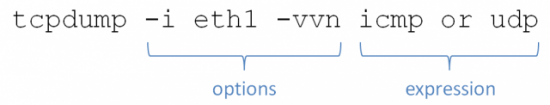
\includegraphics[width=0.5\textwidth]{figures/tcpdump_cmd.png}
    \caption{Структура на tcpdump команда.}
    \label{tcpdump_cmd_fig}
  \end{figure}

  \item \textbf{Цена} Тъй като програмата се разработва на принципа на отворения
    код, тя е изцяло безплатна и може да се използва според BSD лиценза.
  \item \textbf{Програмна поддръжка} Тъй като програмата се разработва на
    принципа на отворения код, тя няма формална поддръжка --- тя се
    базира на обществото от потребители на програмата.
  \item \textbf{Поддръжка на операционната система} Поддържа повечето
    UNIX-базирани операционни системи: Linux, Solaris, BSD, HP-UX и др.
    Microsoft Windows се поддържа през WinDump, която използва
    WinPcap --- Microsoft Windows имплементацията на libpcap.
\end{itemize}


\begin{figure}[h!]
  \centering
  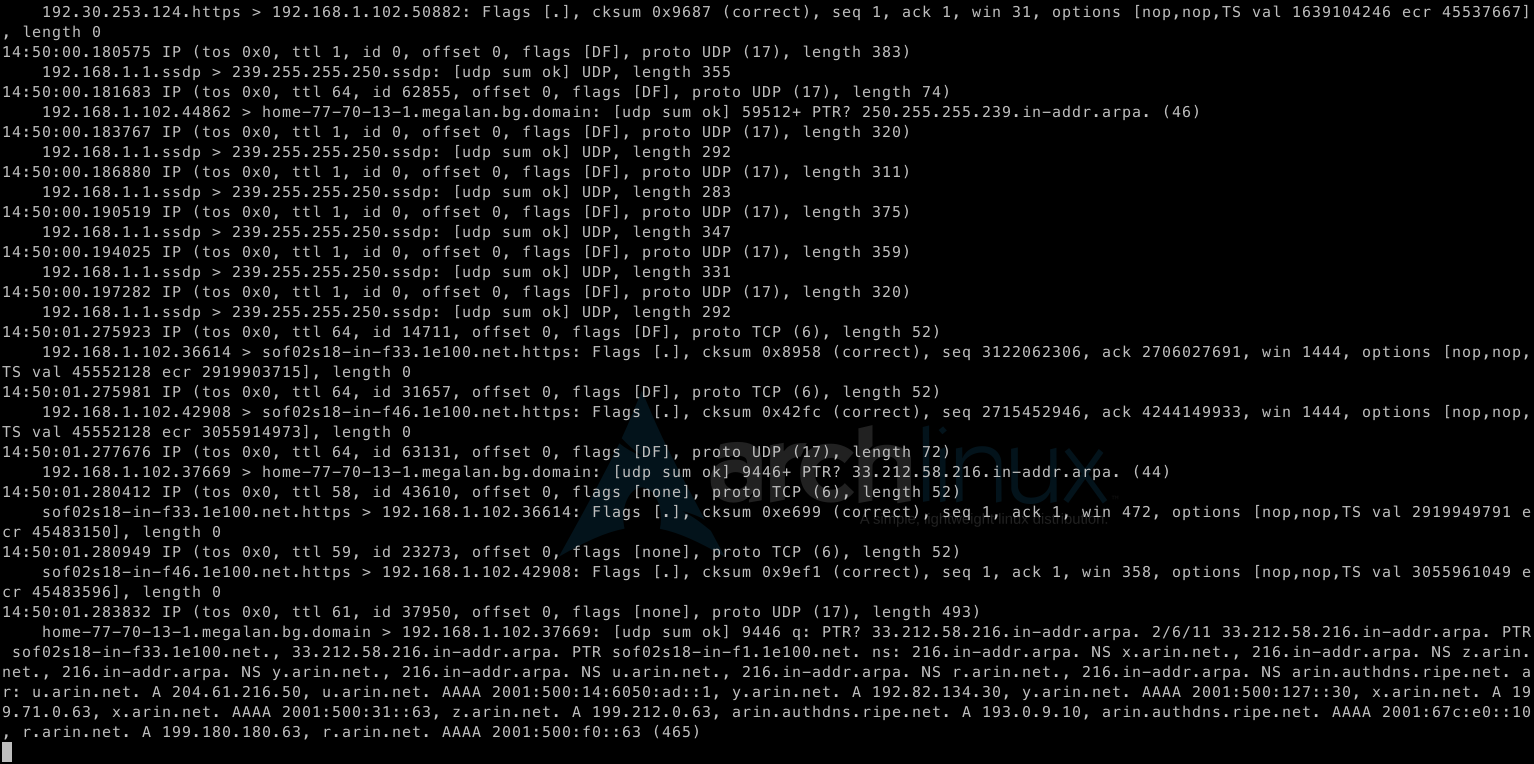
\includegraphics[width=1.0\textwidth]{figures/tcpdump.png}
  \caption{Изглед на потребителския интерфейс на tcpdump.}
  \label{tcpdump_fig}
\end{figure}

\chapter{Проектиране на структурата на мрежов анализатор}

\section{Функционални изисквания към мрежов анализатор}

\subsection{Намиране и избиране на мрежови интерфейси}

Преди да започне какъвто и да било анализ, мрежовия администратор трябва да
получи списък с интерфейси поддържани от мрежовата карта. Списъкът трябва да
съдържа освен имената на интерфейсите, конфигурираният IP адрес,
мрежова маска, broadcast адрес и адрес на получателя в случай на point-to-point
интерфейс. Анализатора трябва да предостави възможност на администратора за
избор на конкретен интерфейс, от когото да се прихваща трафик.

\subsection{Интерпретиране на данни}

Мрежовия анализатор трябва да може да интерпретира прихваната от преносвателната
среда поредица от байтове. Тъй като типично тя е в двоичен вид, информацията за
съдържанието на пренесения PDU трябва да е в разбираем от администратора вид,
т.е представена като символен низ. Фундаментална е функционалността за
интерпретиране на най-често срещаните протоколи в TCP/IP стекa, а именно
Ethernet, IP, TCP, UDP.

\subsection{Филтриране на анализа}

Прихващането на трафик директно от преносвателната среда предполага огромно
количество данни, особено в случай на голямо количество станции. Следователно,
анализирането без филтър би отнело ненужно време и ресурси. Чрез филтрирането
анализатора трябва да позволи на администратора да се абстрахира от ненужния
трафик, като той може да бъде настроен да приема конкретен тип трафик, например
единствено IP трафик. Освен преди началото на анализ, анализатора трябва да
поддържа възможност за филтриране на вече прихванатите пакети по време на анализа.

\subsection{Отдалечен анализ}

Посредством client-server архитектура, анализатора трябва да поддържа отдалечен
анализ. Клиентът трябва да има възможност да задава команди на сървърa, а той
да ги изпълнява, делегирайки част от тях на анализатора за изпълнение.
Комуникацията между клиента и сървъра трябва да е full-duplex и в реално време с
оглед принципа на работа на мрежовия анализатор.

\subsection{Сигурност на отдалечения анализ}

С оглед сигурността, анализатора трябва да поддържаща TLS/SSL, тъй като
евентуалната липса на поддръжка на криптиран трафик би довела до възможност за
\textit{eavesdropping} на комуникацията между двете и следователно до
анализирания трафик, достигащ до клиента от сървърa.

\subsection{Споделяне на анализа}

Анализатора трябва да има възможност за споделяне на анализа: един
клиент трябва да може да инициира анализираща сесия, към която, веднъж инициирана,
може да се присъединят останалите. Всичките едновременно трябва да получават
прихванатия трафик.

\subsection{Сигурност на споделяне на анализа}

Анализатора трябва да поддържа метод за автентикация, който позволява единствено
ауторизирани мрежови администратори да достъпват текущата сесия на
анализ. Така потребител (независимо злонамерен или не), достигнал случайно до
адресa на уеб сървъра, не би имал възможност да проследи целия трафик на
машината.

\subsection{Графичен интерфейс и визуализация}

Анализатора трябва да поддържа лесен за използване и интуитивен графичен
интерфейс. При създаване на нова сесия на анализ, мрежовия администратор трябва
да има възможност за въвеждане на парола, за избиране на физически интерфейс, за
въвеждане на филтри и стартиране на анализатора. Прозорецът на сесията трябва да
съдържа списък с прихванати пакети и кратка информация за тях, както и
компонент показващ детайлното съдържание на избран пакет, представяйки цялата му
структура в интуитивен за разбиране от начинаещ вид.

\section{Съображения за избор на програмни средства и развойна среда}

\subsection{libpcap}

libpcap е библиотека, предоставяща платформенно-независим API с цел
елиминиране на нуждата от системно-зависими модули в приложенията на по-високо
ниво, тъй като всяка операционна система имплементира свои собствени такива
механизми. Откъм операционни системи, libpcap се поддържа на повечето UNIX-базирани
операционни системи --- Linux, Solaris, BSD и др. Съществува и разновидност за
Microsoft Windows --- winpcap. Взимайки предвид разновидността от
операционни системи, чрез интерфейса си, libpcap предоставя на мрежовия анализатор
универсалност спрямо ОС на която се изпълнява, което го прави широко приложим.

\subsection{C\texttt{++}}

Езикът C\texttt{++} е език с общо предназначение, използван предимно в сферата на
системното програмиране. Създаден през 1979г. от Бьорн Строуструп, езикът е
комбинация от механизмите за абстракция на Simula и бързината и
ефективността на C. Отчитайки поддръжката на системно програмиране,
програмния код написан на C\texttt{++} лесно взаимодейства със софтуер написан
на други езици. Тази необходимост от взаимодействие е отчетена още от началия
етап на дизайна на езика и поддръжката на C, Assembler и Fortran не изисква
допълнително процесорно време или преобразуване на структурите от данни
\cite{stroustrup_c++_2013}. Тъй като libpcap библиотеката е имплементирана на C,
а C\texttt{++} предоставя широка гама от механизми за абстракция
\cite{stroustrup_c++_2013} на нивото на бързодействие на C, езикът е подходящ за
реализацията на бърз, но и гъвкав мрежов анализатор с възможност за
лесно разширение на съществуващата функционалност.

\subsection{WebSocket и websocketpp}

WebSocket протокола предоставя ефикасно решение на проблема за двустранна комуникация в
реално време, тъй като при него не е необходимо отварянето на множество HTTP връзки
(например посредством \texttt{XMLHttpRequest} обекта, \texttt{<iframe>} или
\textit{long polling}). Предимствата на такъв тип комуникация са значими за
ефективната реализация на отдалечен преглед на анализа в реално време.

За програмната реализация на протокола се използва библиотеката
websocketpp\footnote{\url{https://github.com/zaphoyd/websocketpp}},
основните предимства на която са лесната й интеграция: тя е \textit{header-only}
библиотека, т.е за ползването й е необходимо единствено добавянето на
необходимите \texttt{.h} файлове чрез \texttt{\#include} директивата,
поддържката на TLS и поддръжката на многонишковост.

\subsection{Angular 2}

Angular 2 е втората версия на една от двете най-популярни
(\autoref{top_front_end_frameworks_popularity_fig}) платформи за
разработка на клиентски приложения -- AngularJS. Разработени от два гиганта в IT
индустрията, съответно Google и Facebook, Angular и ReactJS имат някои
съществени разлики.

\begin{figure}[h!]
  \centering
  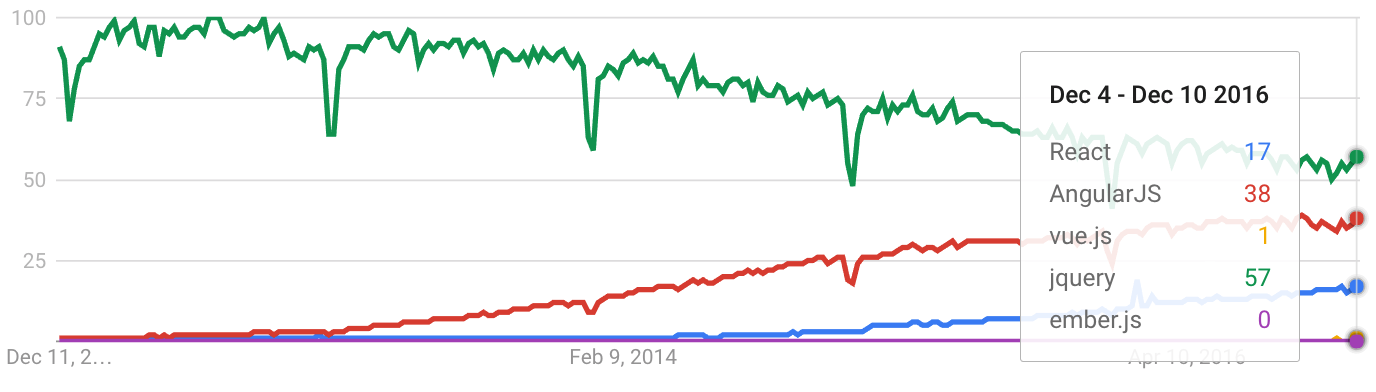
\includegraphics[width=1.0\textwidth]{figures/top_front_end_frameworks_popularity.png}
  \caption{Извадка на най-често търсените JavaScript платформи за разработка на
  потребителски интерфейс. Източник: Google Trends.}
  \label{top_front_end_frameworks_popularity_fig}
\end{figure}

Angular представлява framework, а ReactJS --- библиотека.
ReactJS се концентрира повече върху манипулацията на DOM дървото,
правейки я бърза и ефективнa чрез концепцията за \textit{виртуален DOM}, както и върху
използването на елементи от функционалната парадигма за контрол на състоянието
на приложението чрез шаблони като Flux и Redux. Angular 1.x и неговия наследник
се концентрират повече върху разработката на големи бизнес-ориентирани
приложения, чрез вградена поддръжка на познати концепции от
обектно-ориентираното програмиране като инжектиране на зависимости (dependency
injection), услуги (services)
и компонентно тестване (unit testing). Angular 2.0 има основното предимство, че освен че
надгражда и оптимизира предишната версия, предполага използването на TypeScript.
Взимайки предвид статичната типизация на TypeScript, разработката на едно
Angular 2.0 приложение се улеснява значително поради възможността за статичен
анализ на кода и компилацията \cite{gechev_switching_2016}, водещи до значително
по-малко грешки, а и по-добрата интеграция със средите за разработка.

За програмната реализация на потребителския интерфейс на клиента, освен Angular
се използва angular-seed\footnote{\url{https://github.com/mgechev/angular-seed}},
даващ наготово разделяне на средата за разработка (development) от
продуктовата среда (production), както и интеграция на Angular 2 с някои
популярни инструменти, улесняващи допълнително разработката --- gulp,
Livereload и др.

\section{Проектиране на архитектура на мрежов анализатор с отдалечен достъп}

\subsection{Цялостна архитектура}

На \autoref{client_server_abstract_fig} е представен абстрактен поглед върху
цялостната архитектура на приложението. Със стрелките е означен потока от
данни между клиентите (мрежовите администратори), сървърът и анализаторът. След
като е прихванат от преносвателената среда, пакетът се обработва, подава на
сървъра и бива изпратен до всички автентикирани клиенти (broadcast).
Междувременно комуникацията между сървъра и клиентите е двупосочна (full-duplex)
--- те могат да изпращат различни команди, например да се автентикират към сървъра,
да проверят дали съществува сесия, да стартират сесия и т.н.

\begin{figure}[h!]
  \centering
  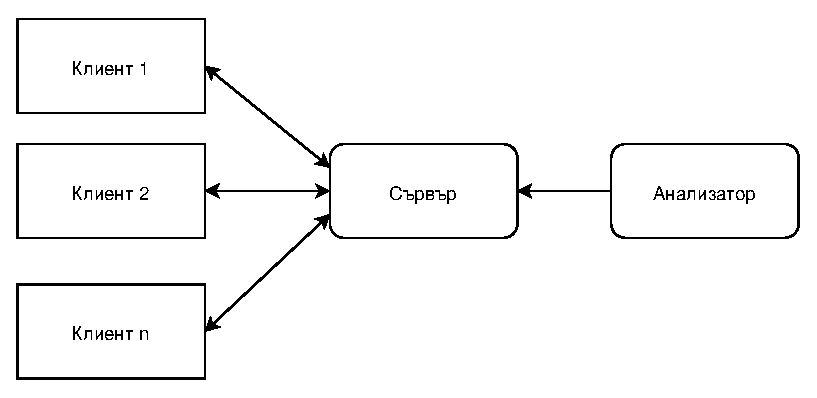
\includegraphics[scale=.7]{figures/client_server_abstract.eps}
  \caption{Абстрактен поглед върху архитектурата.}
  \label{client_server_abstract_fig}
\end{figure}

Важно е да се отбележи, че приложението е многонишково: освен основната нишка,
съществува нишка, обработваща събития на сървъра (например получаване на
съобщение), както и нишка, която извършва реалния анализ.

\subsection{Архитектура на общи класове}

Цялостната архитектура на приложението не би била напълно описана без
споменаването на двата класа \texttt{ConfigurationManager} и
\texttt{SerializationManager}. Те се
занимават съответно с конфигурацията на сървъра и със сериализацията на данните
готови за изпращане до клиента (на практика всички класове, имплементиращи
интерфейс \texttt{SerializableEntity}). Тези два класа представляват характерен пример за т.нар.
\textit{дизайн, базиран на политики} (\textit{policy-based design}),
според когото биха се характеризирали като класове 'гостоприемници' (host
classes).  Парадигмата е
еквивалентна на класическия шаблон за дизайн \textit{стратегия}
(\textit{strategy}) \cite{gamma_design_1995},
отчитайки предимството, че стратегиите
при нея се определят по време на компилация, което намалява разхода на
процесорно време и памет за извикване на виртуални методи.
\cite{alexandrescu_modern_2001}.  На \autoref{configuration_manager_uml_fig} е
представена йерархията на \texttt{ConfigurationManager}. Йерархията на
\texttt{SerializationManager} е аналогична.

\begin{figure}[h!]
  \centering
  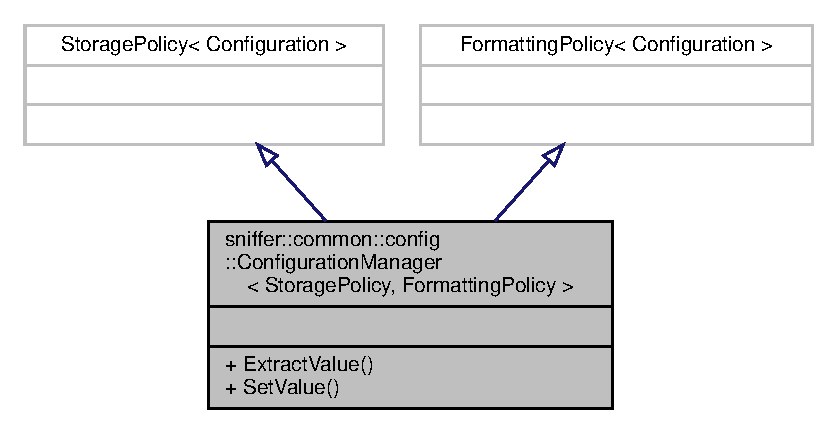
\includegraphics[scale=.7]{figures/configuration_manager_uml.eps}
  \caption{UML диаграма на \texttt{ConfigurationManager} класа.}
  \label{configuration_manager_uml_fig}
\end{figure}

\subsection{Архитектура и алгоритъм на мрежовия анализатор}

В основата на архитектурата на мрежовия анализатор са класовете
\texttt{LayerStack} и \texttt{Layer}. Двата класа представляват частично
модифицирана имплементация на шаблона за дизайн
\textit{протоколен стек}\footnote{\url{http://www.eventhelix.com/RealtimeMantra/PatternCatalog/protocol_stack.htm}}.
Решението, освен разделяне (decoupling) на
отговорността на слоевете, позволява динамична промяна на слоевете на стека,
например ако е нужно 'подпъхване' на междинен слой между два вече съществуващи.
Публичният интерфейс на \texttt{LayerStack} е описан на
\autoref{layer_stack_uml_fig}

\begin{figure}[h!]
  \centering
  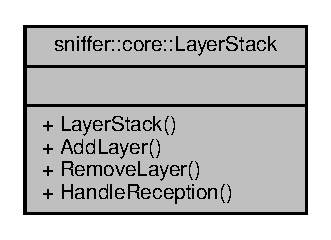
\includegraphics[scale=.9]{figures/layer_stack_uml.eps}
  \caption{UML диаграма на класа \texttt{LayerStack}.}
  \label{layer_stack_uml_fig}
\end{figure}

\texttt{Layer} е базов клас за всички слоеве, както е представено на
\autoref{layers_uml_fig}.  Индивидуалните слоеве се достъпват чрез указатели
от този тип. Предимството е, че конкретния тип на горния и долния слой е
неизвестен за имплементацията на даден слой.

\begin{figure}[h!]
  \centering
  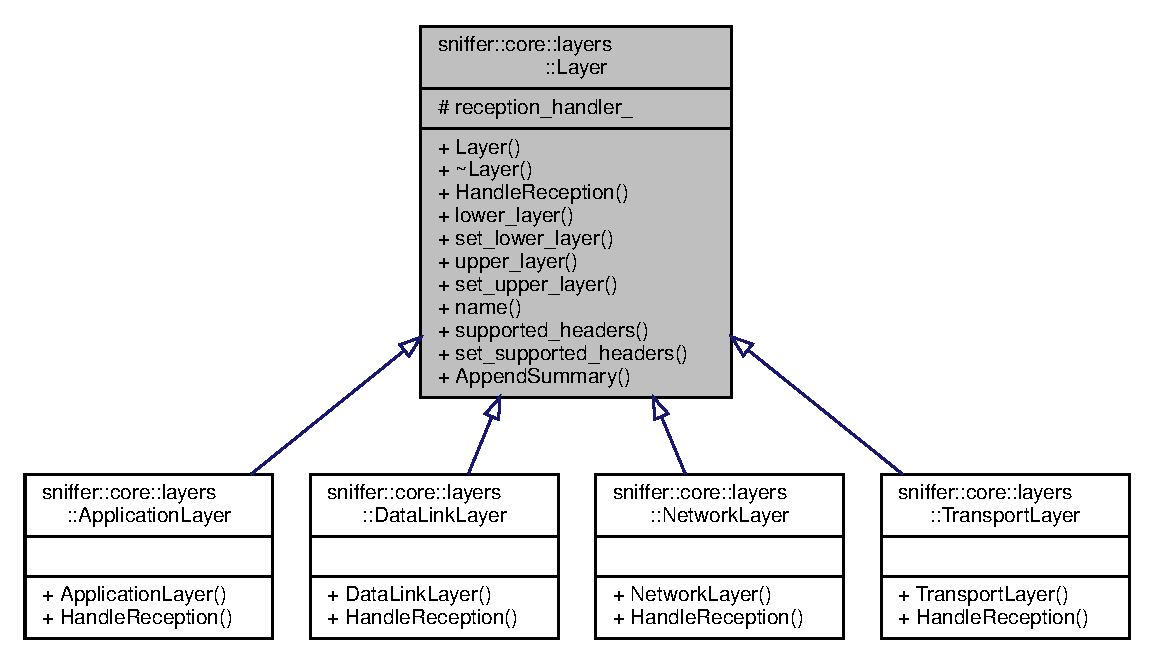
\includegraphics[scale=.7]{figures/layers_uml.eps}
  \caption{UML диаграма на класа \texttt{Layer} и наследниците му.}
  \label{layers_uml_fig}
\end{figure}

Всеки обект от типа \texttt{Layer} има списък от поддържани \texttt{Header}
обекти (представляващи концепцията за заглавна част) посредством обекти от типа
\texttt{HeaderMetadata}. Например, този списък за
\texttt{TransportLayer} би съдържал обекти от типовете
\texttt{UserDatagramHeaderMetadata} и \texttt{TransmissionControlMetadata}.
Всеки \texttt{HeaderMetadata} клас описва някаква метаинформация за
заглавната част,
например дали е с променлива дължина, името на
\texttt{Header} класа, който да се инстанцира, минималната дължина на
съответната заглавна част
и т.н. Всеки \texttt{HeaderMetadata} клас съдържа списък на съответствие между
уникален идентификатор за конкретната заглавна част и името на \texttt{Header}
класа, за когото този идентификатор е валиден.

На \autoref{sniffed_packet_uml_fig} е показан публичният интерфейс на
\texttt{SniffedPacket} класа. Той представлява частнично модифицирана
имплементация на шаблона за дизайн \textit{протоколен
пакет}\footnote{\url{http://www.eventhelix.com/RealtimeMantra/PatternCatalog/protocol_packet_design_pattern.htm}}, още известен като
\textit{протоколен буфер} или \textit{многослоен буфер}. Взимайки предвид
вече описания модел на протоколна комуникация,
всеки слой добавя или премахва своя заглавна или крайна част.
Това предразполага към имплементация, в която всеки слой заделя или освобождава
нов буфер отчитайки новия размер. Изложения шаблон дава просто и ефективно
решение на този проблем.

\begin{figure}[h!]
  \centering
  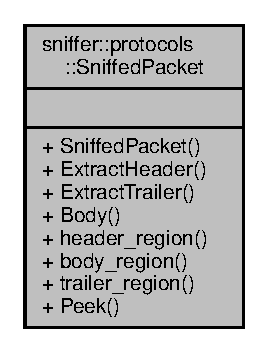
\includegraphics[scale=.7]{figures/sniffed_packet_uml.eps}
  \caption{UML диаграма на класа \texttt{SniffedPacket}}
  \label{sniffed_packet_uml_fig}
\end{figure}

Буферът стандартно се разделя на три области: заглавна (header), основна (body)
и крайна (trailer).
Алгоритъма на декапсулиране, представен визуално на
\autoref{sniffed_packet_regions_fig}, e следния:

\begin{enumerate}
  \item
    Полученият пакет се създава с всички байтове в body областта. В този начален
    момент, header и trailer областите имат нулева дължина.
\item
  Слой 1 изважда своите header и trailer области, двете области се 'отрязват' от
  body областта. Размера на body областта се намалява.
\item
  Слой 2 също изважда своите header и trailer области, двете области отново се
  'отрязват' от body областта. Размера на body областта се намалява.
\item
  Аналогичен е процесът при трети слой, след който се получава изначалната body
  област.
\end{enumerate}

\begin{figure}[h!]
  \centering
  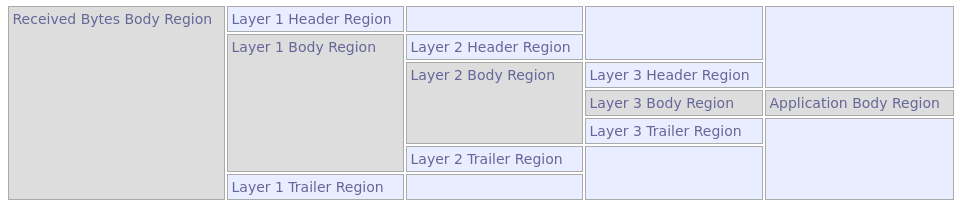
\includegraphics[width=\textwidth]{figures/sniffed_packet_regions.png}
  \caption{Диаграма на разпределение на областите при получаване на пакет.}
  \label{sniffed_packet_regions_fig}
\end{figure}

Представен на \autoref{packet_sniffer_uml_fig} е абстрактния клас
\texttt{PacketSniffer} и имплементацията му \texttt{PcapPacketSniffer}.
Абстракцията е необходима с цел поддръжка на библиотеки на ниско ниво различни
от libpcap.  Публичният интерфейс на класа е тривиален --- метод,
който стартира анализатора, като в имплементацията си извиква последователно
частни виртуални методи за подготовка на физическите интерфейси, за
интерпретиране на заданените филтри и прилагането им, което на практика
имплементира шаблона за дизайн \textit{шаблонен метод} (\textit{template method}).
\cite{gamma_design_1995} Това позволява
различните имплементации на мрежов анализатор да предефинират поведението на
описаните методи необходими за стартиране.
Всеки обект от типа \texttt{PacketSniffer} е композиран от обект от типа
\texttt{LayerStack}. С оглед имплементацията на мрежов анализатор описана в
първа глава, \texttt{LayerStack} е де факто аналогичен, паралелен на системния
протоколен стек, но локален за мрежовия анализатор.

\begin{figure}[h!]
  \centering
  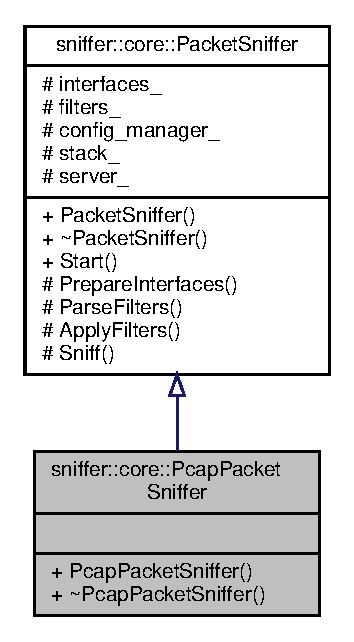
\includegraphics[scale=.7]{figures/packet_sniffer_uml.eps}
  \caption{UML диаграма на класа \texttt{PacketSniffer}.}
  \label{packet_sniffer_uml_fig}
\end{figure}

\subsubsection{Намиране на мрежови интерфейси за анализ}

В основата на функционалността за намиране на мрежови интерфейси
стои класът \texttt{InterfaceRetriever}. Публичният му интерфейс се състои от
един метод --- \texttt{Retrieve()}, който предоставя списък от интерфейси
(\texttt{Interface} обекти) на извикващия. Всеки от тези интерфейси съдържа в
себе си списък от \texttt{InterfaceAddress} обекти, представляващи съответните
адреси за интерфейса, например настроеният IP адрес, мрежова маска,
broadcast адрес и т.н. Информацията е аналогичнa на изхода на \texttt{ifconfig} командата
в UNIX операционните системи.

\texttt{InterfaceRetriever} съдържа обект от типа
\texttt{IpAddressFactory}. Целта на \texttt{IpAddressFactory} е да инстанцира
обекти от типа \texttt{IpAddress} --- типична
имплементация на шаблона за дизайн \textit{завод} (\textit{factory}) \cite{gamma_design_1995}.
Класът \texttt{IpAddress} е базов за класовете \texttt{Ipv4Address} и
\texttt{Ipv6Address}, съответно енкапсулиращи данни за IPv4 и IPv6 адрес.

\subsubsection{Основен алгоритъм на работа}

\begin{figure}[h!]
  \centering
  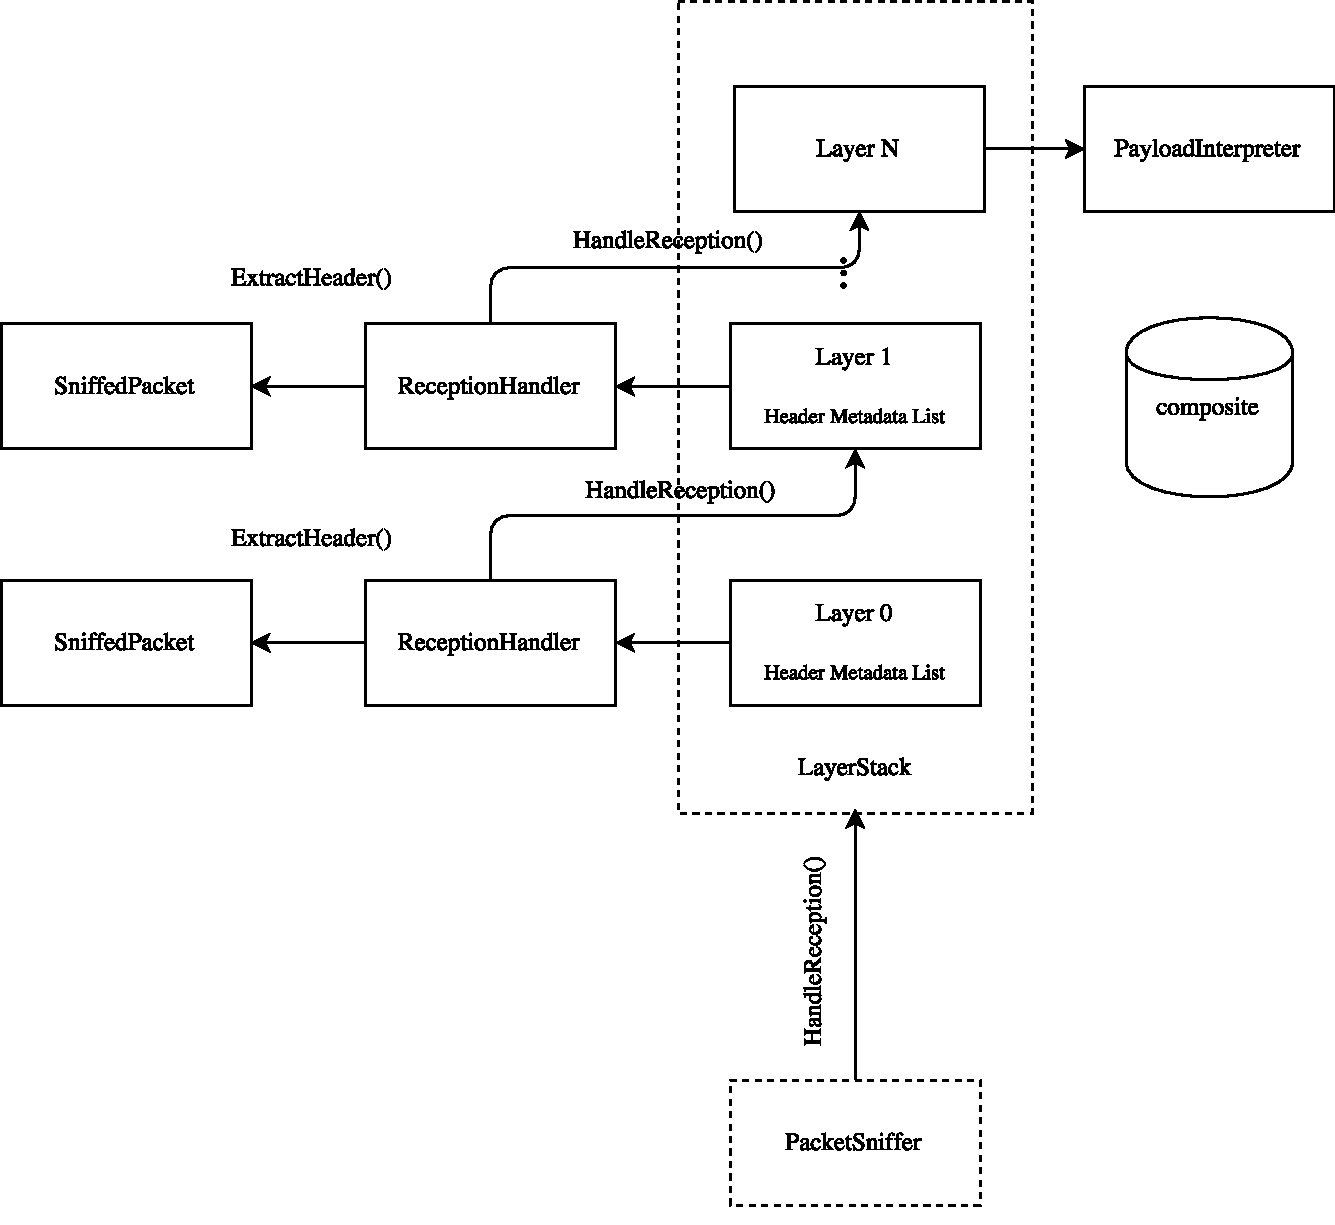
\includegraphics[scale=.7]{figures/main_algorithm.pdf}
  \caption{Основен алгоритъм на работа.}
  \label{main_algorithm_fig}
\end{figure}

Основния алгоритъм се базира на вече описания принцип на работа на протоколната
комуникация, както и на вече описаните основни класове. Класът
\texttt{PacketSniffer} има \textit{callback} метод, който се извиква
в момента на получаване на пакет по преносвателната среда. Инстанцира се обект
от типа \texttt{SniffedPacket}, който бива предаден на протоколния стек. Той го
препредава на най-ниския слой. При предаването, освен \texttt{SniffedPacket} обекта, се
предават три параметъра ---
\texttt{composite}, който представлява дървовидна йерархична структура,
позволяваща 'наслагване' на сериализираните полета на
всеки \texttt{Header}, името на предишния \texttt{Header} обект, обработил пакета, и текущия уникален
идентификационен номер, извлечен от предишния \texttt{Header}. \texttt{ReceptionHandler} обекта
проверява дали на текущия слой съществува \texttt{HeaderMetadata} със зададено
съответствие между името на предишния \texttt{Header} обект и текущия уникален
идентификационен номер. Ако
съществува, инстанцира обект от типа \texttt{Header}, който извлича себе си от
\texttt{SniffedPacket} обекта, сериализира го и го наслагва върху
\texttt{composite}
обекта, препредавайки същите параметри на горния слой, където процеса е
аналогичен. На последния слой същинските данни, енкапсулирани от слоевете, се
интерпретират в някакъв формат и също се наслагват върху \texttt{composite} обекта,
който бива изпратен до всички автентикирани клиенти на сървъра. Ако не
съществува,
\texttt{SniffedPacket} обекта се определя като невалиден и понататъчната
обработка се прекъсва.

\subsection{Архитектура на сървър}

В ядрото на сървърната част на цялостната архитектура е \texttt{Server} класа.
Неговият интерфейс описва абстрактна функционалност за добавяне на нови връзки,
за множествено изпращане (broadcast), за автентикация, за поддръжка на host на
сесията (т.е мрежовия администратор, инициирал сесия на анализ). Абстракцията на
този клас предполага лесна подмяна на \texttt{WebSocketServer} класа, представен
на \autoref{server_websocketserver_uml_fig}, с друг тип
сървър.

\begin{figure}[h!]
  \centering
  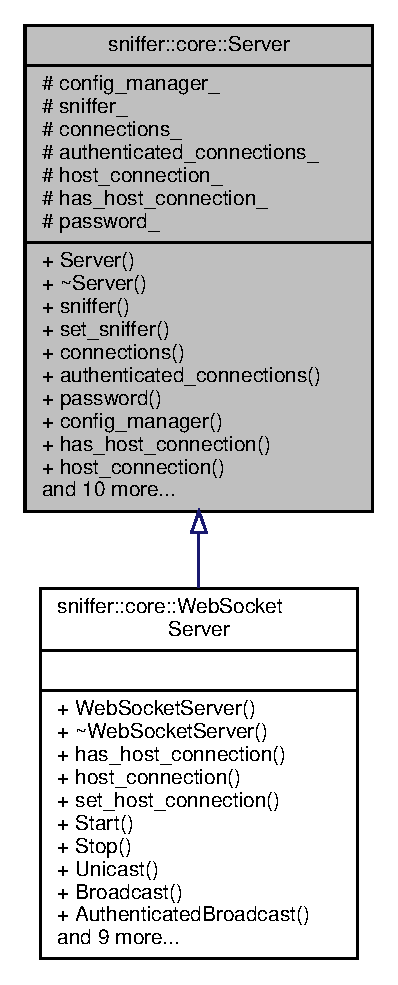
\includegraphics[scale=.7]{figures/server_websocketserver_uml.eps}
  \caption{UML диаграма на класовете \texttt{Server} и \texttt{WebSocketServer}.}
  \label{server_websocketserver_uml_fig}
\end{figure}

\subsubsection{Поддръжка на команди}

Комуникацията между клиентите и сървъра може да бъде разгледана като команди,
които клиентите изпращат и биват съответно изпълнени върху сървърa.
Това предполага имплементацията на класическия шаблон \textit{команда}
(\textit{command}). С това
се цели разделяне (decoupling) на обекта, извикващ изпълнението
(\texttt{ServerCommandInvoker}) и обекта,
действително изпълняващ командата (\texttt{Command}). Това улеснява
добавянето на нови команди чрез просто наследяване на \texttt{Command} класа,
както изложено на \autoref{server_command_uml_fig}.  \cite{gamma_design_1995}.

\begin{figure}[h!]
  \centering
  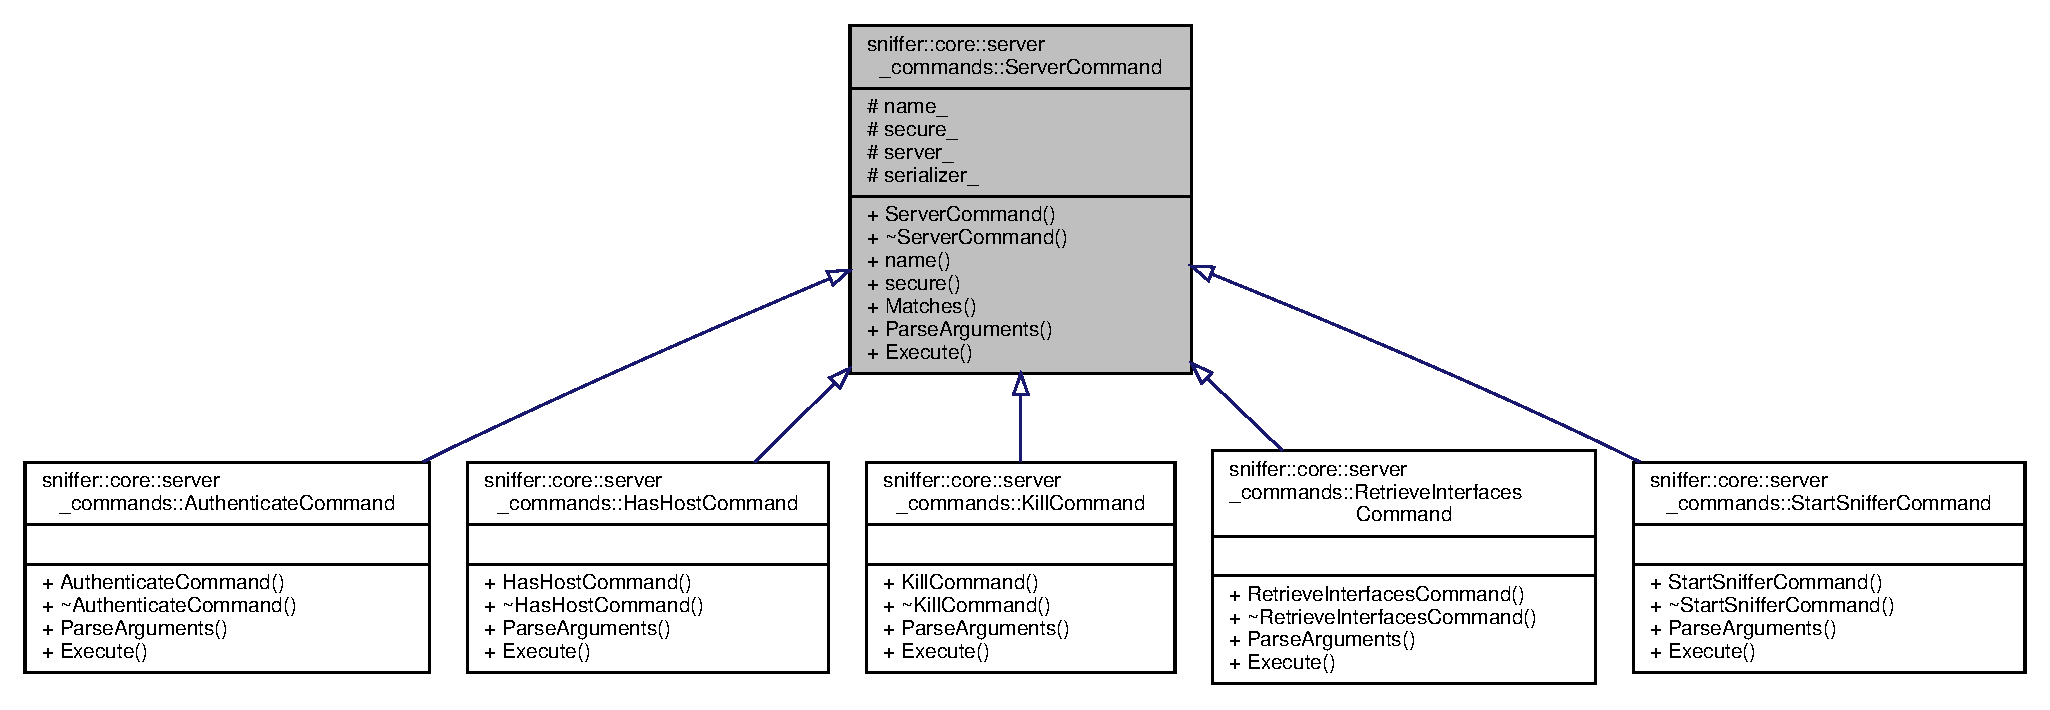
\includegraphics[scale=.5]{figures/server_command_uml.eps}
  \caption{UML диаграма на класа \texttt{ServerCommand} и наследниците му.}
  \label{server_command_uml_fig}
\end{figure}

\subsubsection{Модели на отговор при изпълнени команди}

Изпълняването на дадена команда върху сървъра предполага отговор за състоянието
след изпълнение на командата към клиента. С оглед разделянето на отговорности,
тези класове са обособени в \textit{модели на отговор} (\textit{response models}).
\textit{Модел} тук може да се разглежда като
аналог на моделите при архитектурните шаблони за дизайн от типа на MVC, MVVM и
т.н. Всеки от тях описва някакво състояние, например
\texttt{RetrieveInterfacesResponseModel} има списък от \texttt{Interface}
обекти.

Тривиално, те поддържат метод за сериализацията на модела на отговора с оглед
необходимостта от пренасянето на данните по канала между клиента и сървъра.

\subsection{Архитектура на клиент}

\subsubsection{Компонентно дърво}

Базирайки се на компонентната архитектура на Angular 2, архитектурата на
приложението има следния йерархичен вид:

\begin{figure}[h!]
  \centering
  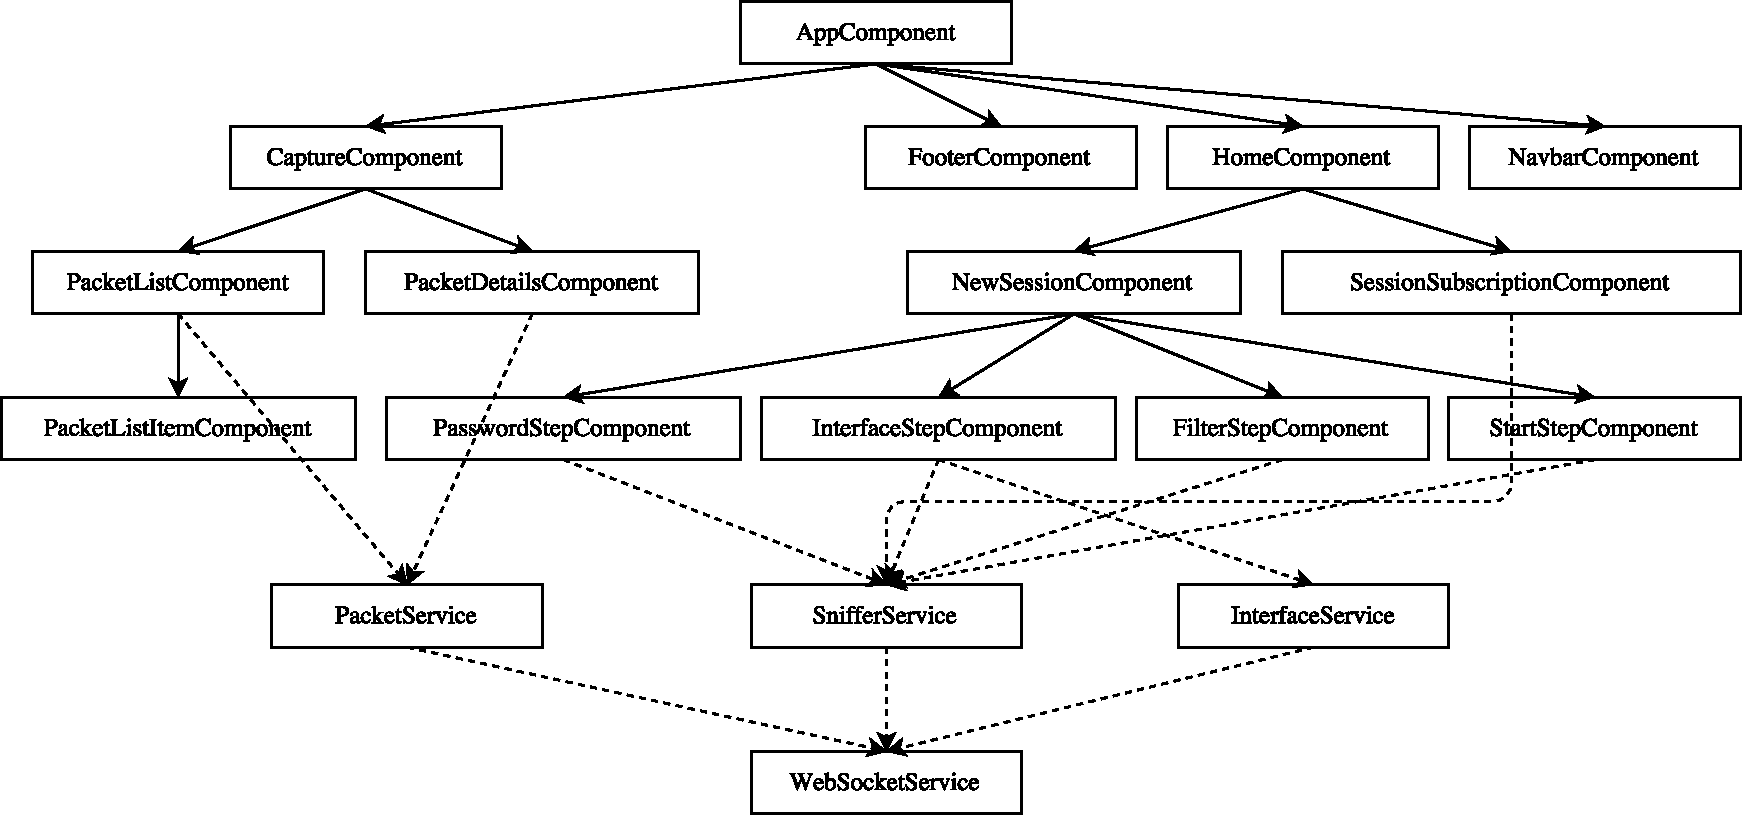
\includegraphics[scale=.5]{figures/ng_component_and_dependencies_tree.pdf}
  \caption{Компонентно дърво на потребителския интерфейс и зависимости на
  компонентите от услугите.}
  \label{ng_component_and_dependencies_tree_fig}
\end{figure}

Потребителския интерфейс е съставен от два основни компонента:
\texttt{HomeComponent} и \texttt{CaptureComponent}. \texttt{HomeComponent}
има две деца: \texttt{NewSessionComponent} и \texttt{SubscriptionComponent}.
Първото представлява компонента за създаване на нова сесия на анализ, т.е когато
когато клиентът е установил, че никой друг не е инициирал такава. То поддържа
подстъпки за въвеждане на парола, избиране на интерфейси, въвеждане на филтър и
стартиране на сесията на анализ, които са енкапсулирани в отделни компоненти.
\texttt{SubscriptionComponent} компонента се инициализира в случаите, когато
сесия на анализ съществува и втория (в общия случай \textit{n}-тия) мрежов администратор
я достъпва. Стандартно този компонент предоставя възможност за въвеждане на
парола.

\texttt{CaptureComponent} представлява реалния екран на анализ, т.е като
подкомпоненти поддържа списък с пакетите, които са получени от сървъра (и
съответно анализатора), детайли за избран пакет във вид на йерархична
структура, както и компонента \texttt{PacketBytesComponent} (липсва на
\autoref{ng_component_and_dependencies_tree_fig}), който има
тривиалната функция да покаже получената от сървъра интерпретация на полезната
информация в даден пакет като текст. Като цяло \texttt{CaptureComponent} е
взаимстван от основния екран на Wireshark.

На \autoref{ng_component_and_dependencies_tree_fig} също са маркирани
(с прекъсната линия) зависимостите на компонентите от съответните
\textit{услуги} (\textit{services}). Услугите енкапсулират т.нар.
\textit{бизнес логика} като съответно биват разделени (decoupled) от
генерирането на потребителския интерфейс. Това улеснява компонентното тестване
на всеки от тях, както и подмяната им (mocking).

Ядрото на клиента е \texttt{WebSocketService} услугата. Тя енкапсулира
извикванията към WebSocket API на браузъра в удобен интерфейс. От нея зависят
услугите, от които клиентът достъпва получените пакети (\texttt{PacketService}) и
физическите интерфейси (\texttt{InterfaceService}). \texttt{PacketService} също поддържа
възможност за избиране на 'наблюдяван пакет', който се настройва
когато администратора избере един пакет от главния списък, както и филтрация на пакети. \texttt{SnifferService}
представлява абстракция върху командите, които могат да се изпълнят на сървъра,
т.е метода \texttt{retrieveInterfaces()}, изпълнен върху обект от тип
\texttt{SnifferService}, би изпратил команда за намиране и извличане на
физическите интерфейси. Отговора от командата би бил наличен през
\texttt{InterfaceService}.

Голяма част от дизайна на услугите е базиран основно на
парадигмата \textit{реактивно програмиране}, използваща т.нар.
реактивни разширения (reactive extensions), реализирани чрез
RxJS библиотеката, вградена в Angular 2. На практика,
те позволяват програмиране с асинхронни потоци от събития или данни,
като предимството е, че в тях е застъпена функционалната парадигма,
следователно тези потоци могат да се съединяват (merge), филтрират,
трансформират (map) и др.
Пример\footnote{\url{https://gist.github.com/staltz/868e7e9bc2a7b8c1f754}} за поток може да бъде стандартно \texttt{click}
събитие:

\begin{figure}[h!]
  \centering
  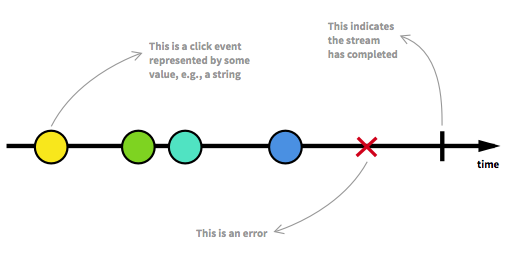
\includegraphics[width=0.5\textwidth]{figures/observable.png}
  \caption{Визуализация на асинрхонен поток от данни.}
  \label{observable_fig}
\end{figure}

Всяко събитие се прихваща асинхронно чрез дефиниране на callback
функция, изпълняваща се при излъчване на стойност, на друга подобна
функция, изпълняваща се когато е излъчена грешка, и на друга такава,
когато е излъчено събитие за край
на потока (completed). Тези функции се наричат изследващи състоянието
(observers), а потока, който се изследва --- изследваем (observable). В
обектно-ориентирания дизайн този шаблон е известен като \textit{наблюдател}
(observer). \cite{gamma_design_1995}

\chapter{Програмна реализация на мрежов анализатор}

\section{Имплементация на общи класове \texttt{ConfigurationManager} и
\texttt{SerializationManager}}

\subsection{Имплементация на клас, енкапсулиращ конфигурация}

Конфигурацията е имплементирана чрез класа \texttt{Configuration}, чиято
единствена цел е да енкапсулира съдържанието й във вида на символен низ.

\lstinputlisting[language={[11]C++}, caption={Дефиниция на
  \texttt{Configuration} класа}, firstline=30,
lastline=38, linerange={30-38}]{../sniffer/src/common/include/common/config/configuration.h}

Имплементацията на класа е тривиална: съдържа инициализация на частното поле,
както и метод за достъпването му, поради което не е представена.

\subsection{Имплементация на \texttt{ConfigurationManager}}

Класът \texttt{ConfigurationManager} е клас 'гостоприемник' (host class) на
различни политики.  Целта му е да предостави функционалност за извличане и задаване на стойност
от или на конфигурация. Типично една конфигурация представлява йерархична
структура от вида:

\begin{lstlisting}[caption=Пример за формат на конфигурация]
{
    "sniffer": {
        "snap_len": 1518
    },
    "server": {
        "port": 1903,
        "password": "foo",
    }
}
\end{lstlisting}

В случая е използван JSON (Javascript Object Notation) форматът,
но в действителност гъвкавата имплементация позволява използването на
аналогичен йерархичен формат.

Следвайки класическата имплементация на подобен тип класове, класът приема две
политики като аргументи на шаблона: \texttt{StoragePolicy} и \texttt{FormattingPolicy}.
\texttt{StoragePolicy} дефинира начина, по
който конфигурацията се запазва --- във файл, в мрежата и т.н.
\texttt{FormattingPolicy}
дефинира формата на конфигурационния файл --- JSON, XML и т.н.

Класът има два метода: \texttt{ExtractValue()} и \texttt{SetValue()}.  Методът \texttt{ExtractValue()} приемa три
аргумента: тип на стойността, която да прочете, името на обектa
и името на ключa, от които да я извади.
След като вземе пътят към ресурса от политиката за запазване на конфигурацията
и го конкатенира с характерното разширение на политиката за форматиране на
конфигурацията, конфигурацията се чете от политиката за запазване.
Като резултат от метода се извиква политиката за форматиране, към която се делегират параметрите.

\lstinputlisting[language={[11]C++}, caption={Имплементация на
  \texttt{ExtractValue()} метода}, firstline=47,
lastline=56]{../sniffer/src/common/include/common/config/configuration_manager.h}

Методът \texttt{SetValue()} има три параметъра: типа на стойността,
която да запише,
името на обект и името на ключа, в които да се запише дадената стойност. След
като вземе пътят към ресурса от
политиката за запазване на конфигурацията и го конкатенира с характерното
разширение на политиката за форматиране на конфигурацията,
старата конфигурация се чете от политиката за запазване. Новата конфигурация се
генерира посредством политиката на форматиране и базирайки се на старата конфигурация. Накрая
се запазва посредством политиката на запазване.

\lstinputlisting[language={[11]C++}, caption={Имплементация на
  \texttt{SetValue()} метода}, firstline=65,
lastline=77]{../sniffer/src/common/include/common/config/configuration_manager.h}

\subsection{Имплементация на \texttt{FileStoragePolicy}}

Класът \texttt{FileStoragePolicy} представлява политика за запазване на обект от
даден тип \texttt{T} (в случая \texttt{Configuration}) на файловата система.
Той има три метода: \texttt{Read()}, \texttt{Write()} и
\texttt{resource\_path()}.
\texttt{Read()}
метода отваря файла във входен поток, чете съдържанието му, с което
инстанцира обект от типа \texttt{T} (в случая \texttt{Configuration}).
\texttt{Write()} метода отваря изходен поток към файла, чете съдържанието на
обекта от тип \texttt{T} и го пренасочва към изходния поток. Накрая затваря
потока.  \texttt{resource\_path()} връща пътя към файла, в който да се
запази обекта. Методите използват стандартните потоци за вход и изход, затова и
не са представени.

\subsection{Имплементация на \texttt{JsonFormattingPolicy}}

Класът \texttt{JsonFormattingPolicy} представлява политика за форматиране на
обекти от тип \texttt{T}, в случая \texttt{Configuration}, в JSON. Класът на
практика енкапсулира извиквания на функции на
библиотека\footnote{\url{https://github.com/nlohmann/json}} за работа с JSON,
към която делегира същинската обработкa. Има два метода:
\texttt{ExtractValue()}
и \texttt{SetValue()}.

\texttt{ExtractValue()} извлича стойност от даден обект
(в случая \texttt{Configuration}) като го интерпретира в обект от типа
\texttt{nlohmann::basic\_json},
върху когото прилага
\texttt{operator[]()}\footnote{\url{https://nlohmann.github.io/json/classnlohmann_1_1basic__json_a233b02b0839ef798942dd46157cc0fe6.html}}
и шаблонния метод
\texttt{.get<U>}\footnote{\url{https://nlohmann.github.io/json/classnlohmann_1_1basic__json_a16f9445f7629f634221a42b967cdcd43.html}}.

\lstinputlisting[language={[11]C++}, caption={Имплементация на
  \texttt{ExtractValue()} метода на \texttt{JsonFormattingPolicy}}, firstline=46,
lastline=51]{../sniffer/src/common/include/common/config/json_formatting_policy.h}

\texttt{SetValue()} задава стойност на даден обект (в случая
\texttt{Configuration}), като го интерпретира в обект от типа
\texttt{nlohmann::basic\_json}, върху когото прилага вече споменатият
\texttt{operator[]()}, присвоявайки стойността.

\lstinputlisting[language={[11]C++}, caption={Имплементация на
  \texttt{SetValue()} метода на \texttt{JsonFormattingPolicy}}, firstline=65,
lastline=74]{../sniffer/src/common/include/common/config/json_formatting_policy.h}

\subsection{Имплементация на клас, енкапсулиращ сериализиран обект}

Концепцията за сериализиран обект е имплементирана чрез класa
\texttt{SerializedObject}, чиято
единствена цел е да енкапсулира съдържанието на обекта във
вида на символен низ. Имплементацията на класа е тривиална: инициализация на частното поле,
и методи за достъпването му, поради което не е представена.

\subsection{Имплементация на \texttt{SerializationManager}}

Класът \texttt{SerializationManager} е клас 'гостоприемник' (host class)
на различни политики.  Целта му е да предостави общ интерфейс за сериализация
на обекти: създаване на обект, задаване на свойствата му,
добавяне на други обекти, наслагване на обекти и т.н.

Следвайки класическата имплементация на подобен тип класове, класът за момента
приема една политика като аргумент на шаблона: \texttt{SerializationPolicy},
която дефинира конкретния начин на сериализация на обектите --- JSON, XML и т.н.

Имплементацията на класа включва единствено делегиране на същинската
функционалност към
\texttt{SerializationPolicy} класа, затова и не е представена. Обяснение на
принципа на работа на методите на класа е изложено в
имплементация на \texttt{SerializationPolicy} ---
\texttt{JsonSerializationPolicy}.

\subsubsection{Имплементация на \texttt{JsonSerializationPolicy}}

Класът \texttt{JsonSerializationPolicy} представлява политика за сериализация на
обекти от тип \texttt{T}, в случая \texttt{SerializedObject}. Класът на
практика енкапсулира извиквания на функции на вече споменатата
библиотека за работа с JSON, към която делегира същинската обработкa.
Методите \texttt{Create()}, \texttt{ObjectExists()}, \texttt{IsEmpty()}
представляват тривиални методи за създаване на нов обект, проверка дали
свойство на обект съществува и дали на обект липсват свойства. Методите
\texttt{ExtractValue()} и \texttt{SetValue()} представляват подобни по
функционалност методи на вече описаните такива в \texttt{JsonFormattingPolicy}.
Методът \texttt{SetObject()} дава функционалност за вложен обект, т.е един
\texttt{SerializedObject} може да бъде добавен като свойство на родителски
\texttt{SerializedObject}.  \texttt{AppendObject()} има аналогична
функционалност с разликата, че при него вложения \texttt{SerializedObject} се
добавя към свойство на родителския обект от тип масив.

По-интересна е имплементацията на методите \texttt{AppendVariableDepthObject()} и
\texttt{InsertObjectAtNthDepth()}. Спрямо обяснения основен алгоритъм на
реализация, обработвания пакет се 'изкачва' по слоевете на стека. Тези методи
служат за генериране на дървовидната структура на \texttt{composite} обекта,
представляващ сериализирания вариант на пакета.

В \texttt{AppendVariableDepthObject()} се извиква
\texttt{InsertObjectAtNthDepth()}, където всъщност се имплементира логиката по
добавяне на обекта.

\lstinputlisting[language={[11]C++}, caption={Имплементация на
  \texttt{AppendVariableDepthObject()} метода}, firstline=170,
lastline=182]{../sniffer/src/common/include/common/serialization/json_serialization_policy.h}

В \texttt{InsertObjectAtNthDepth()} се имплементира рекурсивно обхождане на
дървото, като при всяко рекурсивно извикване на функцията се калкулира
височината му. Целта е обекта да се запише в списъка с деца на обекта, намиращ се на
разстояние \texttt{subtree\_depth\_delta} от листото на дървото
. На \autoref{insert_object_nth_depth_fig} е представена проста визуализация на
процеса. Например, \texttt{IP} обекта би се записал като дете на
\texttt{Ethernet} обекта, тъй
като в действителност \texttt{Ethernet} енкапсулира \texttt{IP}.
Генерирането на такъв тип структура впоследствие позволява удобна визуализация
на цялостната структура на даден кадър.

\begin{figure}[h!]
  \centering
  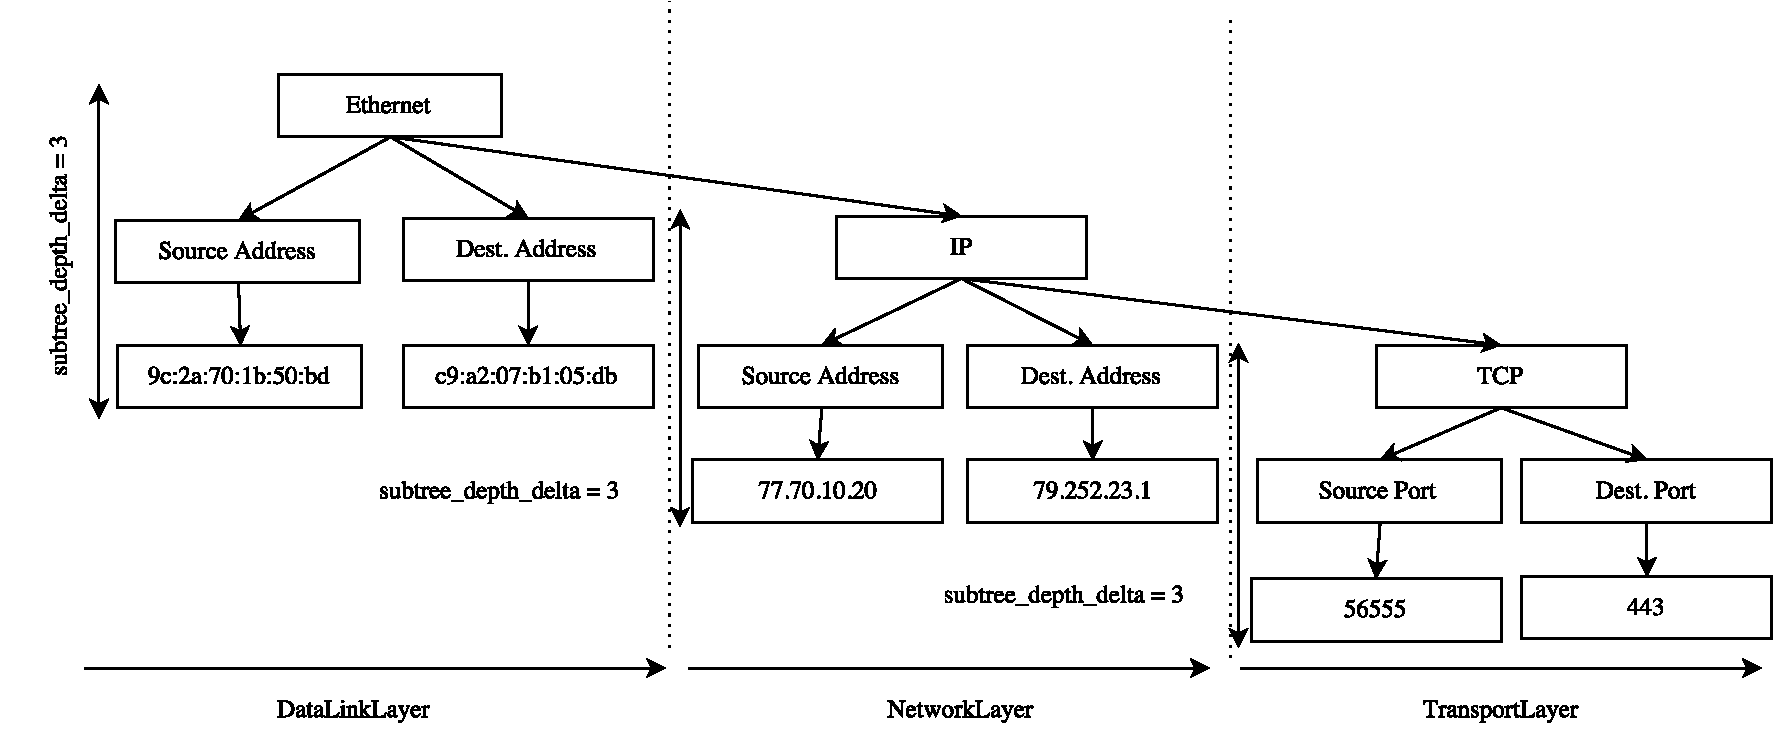
\includegraphics[scale=.5]{figures/insert_object_nth_depth.pdf}
  \caption{Процес на добавяне на нов \texttt{Header} обект към вече изграденото
  дърво.}
  \label{insert_object_nth_depth_fig}
\end{figure}

Описания процес има следната имплементация:

\lstinputlisting[language={[11]C++}, caption={Имплементация на
  \texttt{InsertObjectAtNthDepth()} метода}, firstline=197,
lastline=218]{../sniffer/src/common/include/common/serialization/json_serialization_policy.h}


\section{Имплементация на мрежов анализатор}

\subsection{Имплементация на намиране на физически интерфейси}

\subsubsection{Имплементация на \texttt{InterfaceRetriever}}

В представената дефиниция класа има само един метод ---
\texttt{Retrieve()}, който е публичен виртуален метод. Целта му е конкретната
имплементация на наследника да определи по какъв начин се намират интерфейсите
на ниво операционна система.

\lstinputlisting[language={[11]C++}, caption={Дефиниция на
  \texttt{InterfaceRetriever} класа}, firstline=31,
lastline=41]{../sniffer/src/core/include/core/interface_retriever.h}

\subsubsection{Имплементация на \texttt{IpAddressFactory}}

В представената имплементация на \texttt{IpAddressFactory} методът
\texttt{Parse()} получава указател към структура от тип \texttt{sockaddr}. В
зависимост от стойността на полето \texttt{sa\_family} се инстанцира правилния
обект, съответно енкапсулиращ IPv4 или IPv6 адрес. Методът връща
\texttt{std::unique\_ptr}, тъй като създаващия \texttt{IpAddress} обект е
отговорен за неговото унищожаване. \cite{meyers_effective_2014}

\lstinputlisting[language={[11]C++}, caption={Имплементация на \texttt{Parse()}
    метода на
  \texttt{IpAddressFactory} класа}, firstline=43,
lastline=56]{../sniffer/src/common/src/addressing/ip_address_factory.cc}

\subsubsection{Имплементация на \texttt{IpAddress}}

\texttt{IpAddress} представлява интерфейс съставен от един метод: \texttt{data()},
връщащ указател към началото на масив от символи в паметта, представляващи четим
от човек формат на IP адрес (най-често \textit{dot-decimal} нотация).

\lstinputlisting[language={[11]C++}, caption={Дефиниция на
  \texttt{IpAddress} интерфейса}, firstline=28,
lastline=33]{../sniffer/src/common/include/common/addressing/ip_address.h}

Двете му имплементации: \texttt{Ipv4Address} и \texttt{Ipv6Address} съответно
енкапсулират IPv4 и IPv6 формат на адрес. Тъй като имплементациите са сходни са
представенa само нетривиалната част от имплементацията на \texttt{Ipv4Address}.
Интерфейсът му представлява класически интерфейс на \textit{RAII} (\textit{Resource
Acquisition Is Initialization}) клас: конструктор,
деструктор, копиращ конструктор и копиращ оператор за присвояване
\cite{stroustrup_c++_2013}. Имплементацията на последните три е стандартна и
следователно не е представена. В конструктора се извършва преобразуване на типа
(typecast) на
подадения адрес на \texttt{sockaddr} структура към \texttt{sockaddr\_in}. След
извикването на полулярната
\texttt{inet\_ntop()}\footnote{\url{https://linux.die.net/man/3/inet_ntop}} функция, указателят \texttt{buffer\_}
сочи към масив от символи, съдържащ IPv4 адреса в \textit{dot-decimal} формат.

\lstinputlisting[language={[11]C++}, caption={Имплементация на
  конструктора на \texttt{Ipv4Address} класа}, firstline=43,
lastline=56, linerange={36-40}]{../sniffer/src/common/src/addressing/ipv4_address.cc}

Разликата между \texttt{Ipv4Address} и \texttt{Ipv6Address} е в размера на
буфера, който се заделя в динамичната памет, както и типа на структурата, към
която се извършва преобразуването на типа на \texttt{sockaddr} указателя.

\subsubsection{Имплементация на \texttt{Interface} и \texttt{InterfaceAddress}}

Класът \texttt{InterfaceAddress} енкапсулира логическия адрес на интерфейса,
broadcast адреса му, адреса на получателя (при point-to-point физически интерфейси)
и маската. Включително той поддържа методи за достъп до тези полета.
Освен това, класът имплементира \texttt{SerializableEntity} интерфейса, следвателно има
метод за сериализиране на споменатите полета.

\texttt{Interface} класа описва концепцията за физически интерфейс: той
има име, описание и списък от адреси от тип \texttt{InterfaceAddress}.
Класът също имплементира \texttt{SerializableEntity} интерфейса и следователно
има \texttt{Serialize()} метод, който сериализира името и описанието, итерира
всеки адрес и го сериализира, а след това го наслагва върху основния обект.

\subsubsection{Имплементация на \texttt{PcapInterfaceRetriever}}

Класът \texttt{PcapInterfaceRetriever} е конкретна имплементация на вече
описания \texttt{InterfaceRetriever} за намиране на интерфейси посредством
libpcap библиотеката. В имплементацията на метода
\texttt{Retrieve()}, след намирането на поддържаните мрежови интерфейси от
операционна система посредством
\texttt{pcap\_findalldevs()}\footnote{\url{https://linux.die.net/man/3/pcap_findalldevs}},
характерните за libpcap структури \texttt{pcap\_if\_t} и
\texttt{pcap\_addr\_t}, които абстрактно представляват едносвързан списък, се
итерират и се създават съответните \texttt{Interface} и
\texttt{InterfaceAddress} обекти (полетата на последните посредством
\texttt{IpAddressFactory}).

\subsection{Имплементация на \texttt{LayerStack} и \texttt{Layer} класове}

\subsubsection{Имплементация на \texttt{LayerStack}}

Дефиницията на \texttt{LayerStack} класа включва методи
за добавяне на слой, за премахване на слой и за препредаване на получен пакет
'нагоре' по стека, енумерацията \texttt{Position}, дефинираща къде да бъде поставен даден
слой, и частни полета, пазещи указатели съответно към най-високия и най-ниския
слой на стека.

\lstinputlisting[language={[11]C++}, caption={Дефиниция на
  \texttt{LayerStack} класа}, firstline=50,
lastline=68]{../sniffer/src/core/include/core/layer_stack.h}

Методът \texttt{AddLayer()} добавя слой в стека, като ако такъв не
съществува, новият бива определен като най-високия и най-ниския. Ако такъв
съществува, се взима предвид исканата позиция и съществуващия слой, според които
новият слой се позиционира. Имплементацията е аналогична на имплементацията на
двусвързан списък.

Методът \texttt{RemoveLayer()} премахва слой от стека, като
при премахването свързва слоят над премахнатия с този, който е под него.

Методът \texttt{HandleReception()} има проста имплементация: той предава
получения пакет, както и допълнителните параметри, описани в основния алгоритъм, на
най-ниския слой.

\subsubsection{Имплементация на \texttt{Layer}}

Дефиницията на \texttt{Layer} класа включва метод за получаване на пакет на
слоя (\texttt{HandleReception()}), методи за задаване на горния и долния слой, метод, връщаш
поддържаните \texttt{Header} обекти от слоя (\texttt{supported\_headers()}), и метод, грижещ се за наслагването на обобщена
информация на полетата на даден \texttt{Header} (\texttt{AppendSummary()}) (обобщената информация впоследствие се
използва при показване на листа с пакети на клиента).

\subsubsection{Имплементация на \texttt{Layer} класове}

С оглед изискванията за поддържани протоколи до момента, мрежовия анализатор
има имплементирани четири слоя --- \texttt{DataLinkLayer},
\texttt{NetworkLayer}, \texttt{TransportLayer} и
\texttt{ApplicationLayer}. Имплементацията на първите три е сходна, затова е
представена имплементацията на \texttt{DataLinkLayer}.

\lstinputlisting[language={[11]C++}, caption={Дефиниция на
  \texttt{DataLinkLayer} класа}, firstline=31,
lastline=41]{../sniffer/src/core/include/core/layers/data_link_layer.h}

Класът освен конструктор, приемащ името на слоя и \texttt{SerializationManager}
обекта, който да се използва, има един единствен метод:
\texttt{HandleReception()}. Неговата единствена функция е да делегира приемането
на пакета към \texttt{ReceptionHandler} обект, където се случва реалната
обработка. Именно това е методът, който \texttt{ReceptionHandler} обекта на
долния слой извиква, когато иска да обработи \texttt{Header} предназначен за
горния слой.

По-интересна е имплементацията на \texttt{ApplicationLayer} класа. Тъй като
стандартно той е най-горния слой на стека, в него се случва обработката на
полезната информация, носена от пакета (payload). Като зависимост (dependency)
конструктурът на приложния слой приема \texttt{PayloadInterpreter}, чиито метод
\texttt{Interpret()} извиква за да интерпретира съдържанието на полезната
информация. След което тя се сериализира и съответно наслагва върху
\texttt{composite} обекта.

\lstinputlisting[language={[11]C++}, caption={Имплементация на
  \texttt{HandleReception()} метода на \texttt{ApplicationLayer}}, firstline=58,
lastline=76]{../sniffer/src/core/src/layers/application_layer.cc}

\subsection{Имплементация на \texttt{SniffedPacket} класа}

Както вече описано, \texttt{SniffedPacket} класа е в основата на декапсулацията
на получените по преносвателната среда пакети. Това е имплементирано чрез
структура, описваща обяснените вече области, дефиницията на която включва
полетата \texttt{offset} и \texttt{length}, съответно представляващи изместване
на областта и дължината й:

\lstinputlisting[language={[11]C++}, caption={Дефиниция на
  \texttt{PacketRegion}}, firstline=26,
lastline=32]{../sniffer/src/protocols/include/protocols/packet_region.h}

По-нетривиалните методи на класа \texttt{SniffedPacket} са
\texttt{ExtractHeader()}, \texttt{ExtractTrailer()} и \texttt{Peek()}.
\texttt{ExtractHeader()} се занимава с извиличането на заглавната част, като
съответно формира заглавна област, намалява размера на основната (body) област
и увеличава изместването й.
Аналогично, \texttt{ExtractTrailer()} намалява размера на основната област
и формира крайна област (trailer), започваща от сумата на изместването на основната
област и дължината й. Методът \texttt{Peek()} 'наднича' \texttt{n} байта в body
областта и връща указател, сочещ след тези \texttt{n} байта. Той се използва за извличане на дължините
на заглавните части на пакетите с променлива дължина (такива, при които дължината е кодирана 
като поле на заглавната част), преди да бъде инстанциран конкретния
\texttt{Header} клас.

\subsection{Имплементация на \texttt{ReceptionHandler}}

Класът \texttt{ReceptionHandler} се грижи за изкачването на пакета 'нагоре' по
слоевете и следователно е в центъра на основния алгоритъм.  Методът
\texttt{Handle()} имплементира основната част от логиката. Първоначално той
проверява дали текущия слой поддържа заглавна част, търсейки дали
на слоя съществуват метаданни с подадените (от долния слой) \texttt{prev\_header\_name} и
\texttt{current\_header\_id}. В случай, че се поддържа, от метаинформацията се
взима името на класа на конкретния наследник на \texttt{Header}, изчислява се
дължината му (ако е с променлива дължина, тя се взима чрез
\texttt{SniffedPacket::Peek()}), проверява се дали изчислената дължина не е по-малко от
допустимата, кодирана в метаинформацията. В случай че е, конкретното PDU
(Protocol Data Unit) бива
изхвърлено и понататъчния процес на декапсулация спира. В случай, че не е, се
инстанцира конкретен \texttt{Header} обект, полетата му се сериализират и биват
добавени към \texttt{composite} дървото чрез \texttt{AppendVariableDepthObject()}.
В случай че инстанцирания обект за заглавната част поддържа обобщен вариант на някои негови
свойства, те също се добавят към \texttt{composite} обекта чрез
\texttt{AppendSummary()}
метода на \texttt{Layer}. В края на процеса, ако слоят за когото е създаден
\texttt{ReceptionHandler} обекта има указател към слой над него, пакета
продължава пътя си 'нагоре' по стека като се извиква \texttt{HandleReception()}
метода на горния слой и му се подават името на текущия \texttt{Header} и ID на
следващия.

\subsection{Имплементация на \texttt{PacketSniffer} и \texttt{PcapPacketSniffer}}

\subsubsection{Имплементация на \texttt{PacketSniffer}}

\texttt{PacketSniffer} представлява абстрактен клас описващ мрежов анализатор. В
конструктора той получава необходимите зависимости (dependencies) за анализатора
--- \texttt{LayerStack}, който да ползва при анализирането на пакетите, указател към
\texttt{Server} обекта, интерфейс, филтър и т.н. \texttt{Start()} методът има следната експресивна
имплементация:

\lstinputlisting[language={[11]C++}, caption={Имплементация на
  \texttt{Start()} метода на \texttt{PacketSniffer}}, firstline=55,
lastline=64]{../sniffer/src/core/src/packet_sniffer.cc}

Методите \texttt{PrepareInterfaces()}, \texttt{ParseFilter()} и
\texttt{ApplyFilters()} и \texttt{Sniff()} представляват виртуални методи,
поведението на които конкретните имплементации на мрежов анализатор презаписват
(override).

Същевременно класа енкапсулира нишката, в която се изпълнява мрежовия
анализатор. Тя се стартира чрез \texttt{Run()} метода, а обособяването в метод
е нужно тъй като е възможно при стандартна инициализация в конструктора
нишката да се стартира преди останалите полета да бъдат инициализирани.

\lstinputlisting[language={[11]C++}, caption={Имплементация на
  \texttt{Run()} метода на \texttt{PacketSniffer}}, firstline=69,
lastline=71]{../sniffer/src/core/src/packet_sniffer.cc}

Изпълнението на нишката се спира в деструктора на класа.

\lstinputlisting[language={[11]C++}, caption={Имплементация на
  деструктора на \texttt{PacketSniffer}}, firstline=76,
lastline=80]{../sniffer/src/core/src/packet_sniffer.cc}

\subsubsection{Имплементация на \texttt{PcapPacketSniffer}}

\texttt{PcapPacketSniffer} класа имплементира виртуалните методи на
\texttt{PacketSniffer} чрез libpcap. Методът \texttt{PrepareInterfaces()} първо
намира IPv4 адреса и мрежовата маска за зададения физическия интерфейс чрез
\texttt{pcap\_lookupnet()}, а след това инициализира сесия на анализ чрез
\texttt{pcap\_open\_live()} функцията, която има следния прототип:

\begin{lstlisting}[caption={Прототип на \texttt{pcap\_open\_live()}}]
  pcap_t *pcap_open_live(char *device, int snaplen, int promisc, int to_ms,
        char *ebuf)
\end{lstlisting}

В случая, на функцията се подава избрания физически интерфейс, броя байтове,
които да се заснемат от преносвателната среда, дали интерфейса да е в
\textit{promiscuous} режим, милисекунди за чакане преди да се прочете пакет и указател
към буфер, който се запълва в случай на грешка. Накрая чрез
\texttt{pcap\_datalink()} се прави проверка на типа на протокола поддържан на
каналния слой, в случая всеки различен от Ethernet (DLT\_EN10MB) води до изключение, тъй като е
единствения поддържан от анализатора.

Преди да се приложи даден филтър, той се компилира в \texttt{ParseFilters()} методa чрез
\texttt{pcap\_compile()} функцията:

\begin{lstlisting}[caption={Прототип на \texttt{pcap\_compile()}}]
int pcap_compile(pcap_t *p, struct bpf_program *fp, char *str, int optimize, 
	    bpf_u_int32 netmask)
\end{lstlisting}

Тя приема указател към вече стартирана сесия, указател към мястото, където да се
запази вече компилирания филтър, самия израз за филтрация, дали да се
оптимизира, както и мрежовата маска, върху която да се приложи (която се извлича
в \texttt{PrepareInterfaces()}). Причината да се ползва този метод вместо
стандартни условни конструкции е, че този филтър се оптимизира вътрешно, тъй
като се предава на BPF пакетния филтър.

В \texttt{ApplyFilters()} методa компилирания филтър се прилага чрез
\texttt{pcap\_setfilter()} функцията, приемаща указател към сесия и указател към
компилиран филтър:

\begin{lstlisting}[caption={Прототип на \texttt{pcap\_setfilter()}}]
int pcap_setfilter(pcap_t *p, struct bpf_program *fp)
\end{lstlisting}

След компилация на филтъра, следва пускането на сесията. Това се случва в
метода \texttt{Sniff()}. Той извиква основна функция на libpcap ---
\texttt{pcap\_loop()}:

\begin{lstlisting}[caption={Прототип на \texttt{pcap\_loop()}}]
int pcap_loop(pcap_t *p, int cnt, pcap_handler callback, u_char *user)
\end{lstlisting}

Първият аргумент е указател към сесията, вторият --- колко пакета трябва
функцията да заснеме преди да върне резултат (отрицателна стойност означава
заснемане докато се случи грешка), третият аргумент е името на
\textit{callback} функция, която libpcap да извика, когато заснеме пакет, а
последния: указател към аргументите, които да се подадат на callback
функцията.

В случая, \texttt{pcap\_loop()} се извиква с \textit{callback} функция
\texttt{OnPacketReceived()}, която е статичен метод за класа:

\lstinputlisting[language={[11]C++}, caption={Имплементация на
  \texttt{Sniff()} метода на \texttt{PcapPacketSniffer}}, firstline=118,
lastline=122]{../sniffer/src/core/src/pcap_packet_sniffer.cc}

Важно е да се отбележи, че като аргумент на функцията се подава \texttt{this}
указателя, тъй като в \texttt{OnPacketReceived()} функцията се извиква
метод на класа: \texttt{OnPacketReceivedInternal()}. В него се инициализират
обект от типа \texttt{SniffedPacket}, основната (body) област,
\texttt{composite} обекта, чиито адреси се подават 'нагоре' по стека.

\lstinputlisting[language={[11]C++}, caption={Имплементация на
  \texttt{OnPacketReceivedInternal()} метода}, firstline=147,
lastline=163]{../sniffer/src/core/src/pcap_packet_sniffer.cc}

\subsection{Имплементация на \texttt{Header}, 'формати' за \texttt{Header}
и \texttt{HeaderMetadata}}

\texttt{Header} базовия клас и съответните му наследници представляват
имплементациите на заглавните части на поддържаните протоколи.
Типично всеки \texttt{Header} наследник
приема дължина в конструктора си, извиква \texttt{ExtractHeader()} метода на
\texttt{SniffedPacket} с нея, а
типа на получения указател към начало на заглавната област се превръща
(typecast) към типа на конкретната структура, дефинираща полетата на дадената
заглавна част. Например, в конструктора на \texttt{EthernetHeader}:

\lstinputlisting[language={[11]C++}, caption={Конструктор на
  \texttt{EthernetHeader}},
  firstline=42,
lastline=44]{../sniffer/src/protocols/src/headers/ethernet_header.cc}

Този механизъм се базира на факта че структурите представляват полетата на
заглавната част в десериализиран вид. Имайки точния размер на всяко поле,
съответната клетка от паметта може да бъде десериализирана в поле от структурата.
Този процес е в основата на 'разпознаването' на всеки протокол --- разликата е
единствено във форматът на тези структури за различните протоколи.

Всички такива формати са разделени в
пространството от имена \texttt{sniffer::protocols::headers::formats} и са
дефинирани спрямо стандартните RFC документи за протоколите или съответните
официални стандарти.  Например, TCP има следната стандартна структура от вида:

\lstinputlisting[language={[11]C++}, caption={Формат на заглавната част на TCP},
  firstline=34,
lastline=44]{../sniffer/src/protocols/include/protocols/headers/formats/transmission_control.h}

Освен за десериализиране в конкретни формати, \texttt{Header} наследниците се
грижат за извличането на стойностите от тези структури чрез прилагането на
правилните побитови операции върху полетата, както и за сериализацията им
(\texttt{Header} класа имплементира \texttt{SerializableEntity} интерфейса).

Друг тип фундаментални класове са вече споменатите класове, съдържащи метаданни
за всеки \texttt{Header}. Те са прости класове, съдържащи примитиви за
конкретното име на даден \texttt{Header} клас, за дължината на заглавната част,
за минималната дължина на заглавната част, за отстъплението спрямо началото на
главната част и полето й, където се съдържа информация за дължината й (в случай
на пакети с променлива дължина). Основната структура за всеки такъв тип обаче е
съотвествието между името на заглавната част на по-ниския слой и конкретното ID
на текущата заглавна част за това име, например
\texttt{InternetHeaderMetadata} обект
би имал съответствие от типа: \textit{\string{"EthernetHeader": 0x800\string}},
тъй като \texttt{0x800} е стойността на \texttt{EtherType} полето за IPv4
протокола в заглавната
част на Ethernet кадър.

\subsection{Имплементация на \texttt{PayloadInterpreter} и
\texttt{HexAsciiPayloadInterpreter}}

\subsubsection{Имплементация на \texttt{PayloadInterpreter}}

\texttt{PayloadInterpreter} представлява интерфейс с един метод:
\texttt{Interpret()},
който получава указател към началото на полезната информация в пакета (payload)
и дължината й;

\lstinputlisting[language={[11]C++}, caption={Имплементация на
  \texttt{Interpret()} метода на \texttt{PayloadInterpreter}}, firstline=28,
lastline=33]{../sniffer/src/core/include/core/payload_interpreter.h}

\subsubsection{Имплементация на \texttt{HexAsciiPayloadInterpreter}}

\texttt{HexAsciiPayloadInterpreter} е клас, интерпретиращ полезната информация
на пакета като байтове, представени в шестнадесетична бройна система и ASCII
символи. Той има два метода: \texttt{Interpret()} и \texttt{InterpretLine()}.
\texttt{Interpret()} метода проверява дали дължината на полезната информация е
по-малка от предефинирана константа за брой на байтове на ред
(\texttt{kBytesPerLine}), ако е,
интерпретира само един ред извиквайки \texttt{InterpretLine()}. Ако дължината е
по-голяма, цялата дължина се дистрибутира на редове, дълги
\texttt{kBytesPerLine}, като всеки ред се интерпретира поотделно. Всеки ред има
изместване (\texttt{offset}), което се определя увеличава с \texttt{kBytesPerLine}. Резултата от
интерпретирането на всеки ред се конкатенира в поток от символни низове и e
от вида \textit{\string{{offset   hex   ascii\string}, \string{offset   hex
    ascii\string}, ..,
\string{offset   hex   ascii\string}}}.

\lstinputlisting[language={[11]C++}, caption={Имплементация на
  \texttt{Interpret()} метода на \texttt{HexAsciiPayloadInterpreter}},
  firstline=41,
lastline=75]{../sniffer/src/core/src/hex_ascii_payload_interpreter.cc}

\texttt{InterpretLine()} интерпретира масив от байтове във вида: \textit{offset   hex
ascii}. Алгоритъма използва тривиална указателна аритметика, като единствено инкрементира указателя
\texttt{index\_ptr}, за да трансформира \textit{i}-тия байт чрез
\texttt{std::hex} функцията от стандартната библиотека. Трансформация не се
налага ако \textit{i}-тият байт е ASCII символ.

\section{Имплементация на сървър}

\subsection{Имплементация на \texttt{Server}}

\texttt{Server} класа има сравнително богат публичен интерфейс: методи за
пускане и спиране на сървъра, за спиране на анализатора, за задаване на host връзката (т.е клиентът,
инициирал сесията на анализ), за изпращане на съобщение към конкретен клиент,
към всички клиенти, към всички автенитикирани клиенти, за добавяне на клиент, за премахването му, за
автентикирането на клиент и проверката дали клиент е автенитикиран. Важно е да
се спомене, че клиентът е представен
чрез ID от целочислен тип, т.е конкретните имплементации могат да използват
друг тип, стига той да бъде съпоставим (например чрез \texttt{std::map}) със
съответното ID. Клиентите представляват списък от тези числа, a автенитикацията е имплементирана просто: класът има втори списък
с клиенти, който обаче съдържа само автенитикираните такива. Описаните
вече методи добавят или премахват елементи от съответния списък. По-детайлно
обяснение на методите е представено в наследник на \texttt{Server} класа
--- \texttt{WebSocketServer}.

\subsection{Имплементация на \texttt{WebSocketServer}}

\texttt{WebSocketServer} класа e имплементация на сървър, комуникиращ
посредством WebSocket протокола. Класът енкапсулира \texttt{websocketpp::server}
обект, реализирайки основната си функционалност чрез websocketpp библиотеката.
Освен \texttt{websocketpp::server}, той
съдържа указател към \texttt{WebSocketServerEventHandler} (клас, енкапсулиращ
функционалността за обработка на събития от типа на свързване на нов клиент,
пращане на съобщение от клиент и т.н), съответствие между
\texttt{websocketpp::connection\_hdl} (структура, имплементираща концепцията
за клиент в websocketpp) и целочисления тип, идентифициращ клиенти според
интерфейса на \texttt{Server}, и брояч, определящ следващия ID на
клиент. Състоянието на обект от тип \texttt{WebSocketServer} изисква манипулация от
няколко нишки. Типичен случай, в който \textit{race condition} би се появил е
ако нишката, отговорна за анализа и декапсулация, реши да изпрати обработения
пакет чрез сървъра, докато нишката за обработка на събитията добавя клиент.
С цел избягването на конкурентно модифициране на споделена памет, представените в класа структури биват
предпазени с помощта на популярния принцип за взаимно изключване (mutual
exclusion).

В конструктора на класа се инициализира Boost.Asio библиотеката, която
websocketpp използва за имплементацията си. На \texttt{websocketpp::server} обекта
се задават като \textit{callback} методи методите за обработка на събития на
\texttt{WebSocketServerEventHandler}. \texttt{Start()} методът създава отделна
нишка за обработка на събитията и извиква  \texttt{Run()} метод, частен за
класа, който от своя страна стартира \texttt{websocketpp::server} сървъра. Важно
е да се отбележи, че по този начин на имплементация методите за обработка на
събития на \texttt{WebSocketServerEventHandler}, без \texttt{Handle()} метода, който се изпълнява на
новосъздадената нишка, биват изпълнени на основната нишка на програмата. След
създаването на новата нишка в \texttt{Start()}, се изчаква нейното приключване чрез
\texttt{join()} метода на \texttt{std::thread}. \cite{williams_c++_2012}
Цялостната логика на останалите методи на класа е да изолират критичната секция
чрез мютекс, извиквайки имплементацията на базовия клас (\texttt{Server}).
Например, методът \texttt{AddClient()} добавя клиент по подаден
\texttt{websocketpp::connection\_hdl}.

\lstinputlisting[language={[11]C++}, caption={Имплементация на метода
    \texttt{AddClient()} на
  \texttt{WebSocketServer}}, firstline=252,
lastline=261]{../sniffer/src/core/src/websocket_server.cc}

В случая, списъка на съответствия между \texttt{websocketpp::connection\_hdl} се заключва,
новия клиент се добавя, след което структурата от данни се отключва. Важно е да
се отбележи, че в случая член променливата \texttt{next\_connection\_id\_} няма
нужда от механизъм за взаимно изключване, тъй като \texttt{AddClient()} е
е единствената функцията, променяща стойността й. При инкрементирането й в края
на метода обаче, механизмът е необходим тъй като има вероятност тя да бъде
прочетена в същото време от друга нишка.

\subsection{Имплементация на \texttt{WebSocketServerEventHandler}}

Вече споменатият \texttt{WebSocketServerEventHandler} клас е клас, който
се занимава с логиката по обработка на събитията, свързани със сървъра. Едно
събитие има следната дефиниция:

\lstinputlisting[language={[11]C++}, caption={Дефиниция на структурата
    \texttt{WebSocketServerEvent}}, firstline=31,
lastline=42]{../sniffer/src/core/include/core/websocket_server_event.h}

Вторият конструктор се използва в случай, че събитието е от типа съобщение, в
такъв случай събитието освен тип и клиентът, за когото е валидно, съдържа и
указател към съобщението. Типа
на събитията е енумерация със следната дефиниция:

\lstinputlisting[language={[11]C++}, caption={Дефиниция на енумерацията
    \texttt{WebSocketServerEventType}}, firstline=26,
lastline=26]{../sniffer/src/core/include/core/websocket_server_event_type.h}

Основните методите на класа са \texttt{OnConnectionOpened()},
\texttt{OnConnectionClosed()},
\texttt{OnMessageReceived()}, \texttt{OnTlsInit()} и \texttt{Handle()}.
Първите три метода имат сходна
имплементация, затова е представен само първият:

\lstinputlisting[language={[11]C++}, caption={Имплементация на метода
  \texttt{OnConnectionOpened()}},
  firstline=59,
lastline=69]{../sniffer/src/core/src/websocket_server_event_handler.cc}

Класът \texttt{WebSocketEventHandler} има абстрактна структура от данни
опашка, съставена от събития. При нова връзка, websocketpp извиква въпросният
метод като му подава \texttt{websocketpp::connection\_hdl} за новия клиент.
Опашката се заключва чрез осигурен за нея мютекс, новото събитие се добавя към опашката, тя се отключва, а
нишката за обработка на събитията се сигнализира ('събужда') посредством популярния
механизъм на имплементация с \textit{условна променлива} (condition variable).

\texttt{OnTlsInit()} методът настройва TLS комуникацията между клиента и
сървъра, като конфигурира параметрите й: публичния и частния ключ, типа на TLS
връзката, позволените криптиращи алгоритми и т.н.

\texttt{Handle()} методът, фрагмент от който е представен, изчаква върху условната
променлива главната нишка да сигнализира за пристигнало събитие. При
сигнализация, мютексът се заключва, първото събитие (във FIFO опашката) се изважда, след
това мютексът се отключва, а събитието бива обработено според типа му. Ако
типът му е съобщение, то се интерпретира като изпратена команда, за изпълнението
на която се грижи \texttt{ServerCommandInvoker}.

\lstinputlisting[language={[11]C++}, caption={Част от имплементацията на метода
  \texttt{Handle()}},
  firstline=221,
lastline=229]{../sniffer/src/core/src/websocket_server_event_handler.cc}

\subsection{Имплементация на \texttt{Command}}

Следвайки цялостната архитектура, върху сървъра може да се изпълняват команди.
Концепцията за команда съответства на \texttt{Command} класа, а конкретните
команди просто го наследяват, изменяйки поведението му. Освен указател към
\texttt{Server} обект, върху когото да се изпълни командата, една команда има име
и степен на сигурност (т.е дали може да се изпълнява от неавтентикиран клиент).
Най-фундаменталните методи за класа са: \texttt{Matches()},
\texttt{ParseArguments()} и
\texttt{Execute()}, като последните два са виртуални и конкретните команди определят
поведението им. \texttt{Matches()} метода проверява дали даден символен низ е
команда, като десериализира низа и чрез описаните вече методи за извличане на
стойност в \texttt{SerializationManager} проверява дали обектът има свойство с
името на командата. \texttt{ParseArguments()} връща двойки от ключ-стойност с
името на аргумента на командата и стойността му, по подразбиранe връща празен
\texttt{std::map}. \texttt{Execute()}, логично, изпълнява командата.

\subsubsection{Имплементация на \texttt{AuthenticateCommand}}

\texttt{AuthenticateCommand} сравнява подадената като аргумент на командата
парола с предефинираната парола на сървъра. Инстанцира модел на отговор,
подавайки резултата от предиката, а в случай на съвпадение
--- автенитикира даден клиент към сървъра, т.е. го добавя към вътрешния
списък с автенитикирани клиенти през публичния интерфейс на \texttt{Server}.

\lstinputlisting[language={[11]C++},
  caption={Имплементация на \texttt{Execute()} метода на
  \texttt{AuthenticateCommand}},
  firstline=69,
lastline=81]{../sniffer/src/core/src/server_commands/authenticate_command.cc}

\subsubsection{Имплементация на \texttt{HasHostCommand}}

\texttt{HasHostCommand} проверява дали вече е инициирана сесия на анализ,
резултата от проверката подава на съответния модел на отговор, сериализира го и
изпраща резултата на клиентa, извикал командата.

\subsubsection{Имплементация на \texttt{KillCommand}}

\texttt{KillCommand} спира сървъра като извиква \texttt{Stop()} метода му.

\subsubsection{Имплементация на \texttt{StopSnifferCommand}}

\texttt{StopSnifferCommand} спира сесията на анализ като извиква
\texttt{StopSniffer()} метода на сървъра, в който
\texttt{PacketSniffer} обекта за сървъра се унищожава
(следователно се вика деструкторът на класа), който последователно спира и
нишката, в която се изпълнява анализатора.

\subsubsection{Имплементация на \texttt{RetrieveInterfacesCommand}}

\texttt{RetrieveInterfacesCommand} е командата, която връща списък от физически
интерфейси, поддържащи възможност за анализ. Те са именно интерфейсите, който се
извличат посредством \texttt{InterfaceRetriever} класа. Имплементацията на
\texttt{Execute()} метода е тривиална: извличат се всички интерфейси чрез
указателя към \texttt{InterfaceRetriever}, който е член променлива за командата,
инициализира се модел на отговор, на когото се подават извлечените интерфейси,
той се сериализира и съответно бива изпратен на клиента, изпратил командата.

\lstinputlisting[language={[11]C++},
  caption={Имплементация на \texttt{Execute()} метода на
  \texttt{RetrieveInterfacesCommand}},
  firstline=60,
lastline=69]{../sniffer/src/core/src/server_commands/retrieve_interfaces_command.cc}

\subsubsection{Имплементация на \texttt{StartSnifferCommand}}

\texttt{StartSnifferCommand} инстанцира обект от тип \texttt{PacketSniffer},
подавайки му името на интерфейса и филтъра, който да бъде приложен. В
конкретната имплементация е използван \texttt{PcapPacketSniffer}, но в идеалния случай
аргументът на командата би приемал символен низ, представляващ конкретния тип
\texttt{PacketSniffer}, който да се инстанцира. Изпратилия командата
клиент бива определен като инициатор на сесията за анализ. В нова нишка се
извиква \texttt{Start()} метода на анализатора.

\lstinputlisting[language={[11]C++},
  caption={Имплементация на \texttt{Execute()} метода на
  \texttt{StartSnifferCommand}},
  firstline=87,
lastline=101]{../sniffer/src/core/src/server_commands/start_sniffer_command.cc}

\subsection{Имплементация на \texttt{ServerCommandInvoker}}

\texttt{ServerCommandInvoker} класът има списък от команди, като основния му
метод е \texttt{Invoke()}. Той получава указател към \texttt{Server} обект, върху когото
да изпълни командата, ID на клиента, за когото да я изпълни, и съобщението
получено от клиента в чист вид. Имплементацията на метода е сравнително
експресивна:

\lstinputlisting[language={[11]C++},
  caption={Имплементация на \texttt{Invoke()} метода на
  \texttt{ServerCommandInvoker}},
  firstline=49,
lastline=62]{../sniffer/src/core/src/server_command_invoker.cc}

Проверява се дали полученото съобщение съвпада с регистрирана команда. Ако
командата изисква клиента да е автентикиран, командата се изпълнява тогава и
само тогава, когато клиентът е автентикиран. Ако не изисква автентикация, тя се
изпълнява директно.

\section{Имплементация на клиент}

\subsection{Имплементация на услуги}

\subsubsection{Имплементация на \texttt{WebSocketService}}

Класът \texttt{WebSocketService} се занимава с установяването и поддръжката на
двустранната комуникация със сървъра. Той има два метода:
публичния \texttt{connect()}, и частния \texttt{create()}.
Методът \texttt{connect()} приема URL, към който да се свърже,
създавайки обект от типа \texttt{WebSocket}, дефиниран от WebSocket
API-а на браузъра.

Класът има поле от тип \texttt{Rx.Subject}, което представлява едновременно
изследваем (observable) и изследващ обект (observer) от събития, включващи
съобщение (\texttt{MessageEvent}). Всяка излъчена стойност или
събитие се изпраща на всички изследващи обекти (subscribers). Това
поле се зарежда мързеливо (lazy load) от \texttt{create()} метода.

\lstinputlisting[language={JavaScript},
  caption={Имплементация на \texttt{connect()} метода на
  \texttt{WebSocketService}},
  firstline=12,
lastline=21]{../client/src/client/app/shared/websocket/websocket.service.ts}

В \texttt{create()} метода се създава изследваем обект
(observable), сдвоявайки (bind) callback функциите на изследващия го обект с
тези, извиквани по подразбиране за \texttt{WebSocket} обекта. Така този изследваем
обект на практика приема данните от канала на комуникация и ги 'предава' на
изследващите: когато по канала се получи съобщение, се извиква \texttt{next}
callback функцията на
изследващия, когато се получи грешка --- \texttt{error} callback функцията, когато се затвори
канала --- \texttt{completed} callback функцията.

\lstinputlisting[language={JavaScript},
  caption={Имплементация на \texttt{create()} метода на
  \texttt{WebSocketService}},
  firstline=23,
lastline=43]{../client/src/client/app/shared/websocket/websocket.service.ts}

\subsubsection{Имплементация на \texttt{SnifferService}}

\texttt{SnifferService} поддържа връзка към сървъра, използвайки вече описания
\texttt{WebSocketService}. Вика се \texttt{connect()} метода му с адреса
на сървъра, определен от средата на изпълнение (development или production),
а при отговор потока трансформира получения \texttt{MessageEvent} обект към JSON преди да достигне крайния абонат (subscriber).

\lstinputlisting[language={JavaScript},
  caption={Част от имплементация на конструктора на
  \texttt{SnifferService}},
  firstline=23,
lastline=27]{../client/src/client/app/shared/sniffer/sniffer.service.ts}

Услугата предоставя и методи за 'настройване' на
параметрите на анализатора: тя се инжектира като зависимост (dependency) на
стъпковите компоненти, където последователно тези параметри се настройват --- това
са методите \texttt{interfaceName()} и \texttt{filterExpression()}.
Освен това, тя де факто описва интерфейс към
командите на сървъра, например извикването на \texttt{start()} метода на
\texttt{SnifferService} води до изпращане на команда за стартиране на
анализатора:

\lstinputlisting[language={JavaScript},
  caption={Имплементация на \texttt{start()} метода на
  \texttt{SnifferService}},
  firstline=82,
lastline=93]{../client/src/client/app/shared/sniffer/sniffer.service.ts}

Аналогични са имплементациите на \texttt{retrieveInterfaces()}, \texttt{sendAuthenticate()} и
\texttt{sendHostCheck()} методите. Отговорите на тези команди представляват
потоци:

\lstinputlisting[language={JavaScript},
  caption={Част от имплементация на конструктора на
  \texttt{SnifferService}},
  firstline=29,
lastline=41]{../client/src/client/app/shared/sniffer/sniffer.service.ts}

Те са от типа \texttt{HostInfo} и \texttt{AuthenticationInfo}. Това
на практика са модели, аналогични на моделите на отговор, имплементирани на
сървъра. Потока за отговори на \texttt{retrieveInterfaces()} е енкапсулиран в
друга услуга --- \texttt{InterfaceService}.

\subsubsection{Имплементация на \texttt{InterfaceService}}

Услугата представлява енкапсулация на потока на отговори на командата за
намиране на физически интерфейси, чийто тип е масив от \texttt{Interface}
обекти:

\lstinputlisting[language={JavaScript},
  caption={Имплементация на \texttt{InterfaceService}},
  firstline=8,
lastline=22]{../client/src/client/app/shared/interface/interface.service.ts}

\texttt{Interface} е модел, който дефинира свойствата на един физически
интерфейс. Той е аналогичен по свойства на обектите, към който
\texttt{Interface} обекта на сървъра се сериализира. Има следната дефиниция:

\lstinputlisting[language={JavaScript},
  caption={Дефиниция на \texttt{Interface} моделa},
  firstline=3]{../client/src/client/app/shared/interface/interface.ts}

Подобно на \texttt{Interface}, \texttt{InterfaceAddress} модела на клиента
има свойствата на обекта, резултат от сериализацията на
\texttt{InterfaceAddress} обектите за даден физически интерфейс на сървъра:

\lstinputlisting[language={JavaScript},
  caption={Дефиниция на \texttt{InterfaceAddress} моделa}]{../client/src/client/app/shared/interface/interface-address.ts}

\subsubsection{Имплементация на \texttt{PacketService}}

Класът \texttt{PacketService} предоставя основния поток от пакети, които се
изпращат по комуникационния канал между сървъра и клиента. Стандартно, той бива
трансформиран като се извлечат данните от \texttt{MessageEvent} обекта и се десериализират
в конкретен обект --- \texttt{Packet}. Това става в конструктора на класа:

\lstinputlisting[language={JavaScript},
  caption={Имплементация на конструктора на \texttt{PacketService}
моделa}, firstline=17, lastline=24]{../client/src/client/app/shared/packet/packet.service.ts}

\texttt{PacketService} имплементира и два метода за филтрация на пакети по символен низ,
представляващ JSQL заявка. Филтрацията се извършва чрез библиотеката
searchjs\footnote{\url{https://github.com/deitch/searchjs}},
предоставяща функционалност за изпълняване на SQL-подобни заявки върху колекция
от JSON обекти. В случая, \texttt{filterSingle()} метода приема пакет и
филтриращ израз и връща булева променлива индикираща дали пакета отговаря на
критерия на филтриращия израз.

\lstinputlisting[language={JavaScript},
  caption={Имплементация на \texttt{filterSingle()}
моделa}, firstline=34, lastline=36]{../client/src/client/app/shared/packet/packet.service.ts}

\texttt{filterCollection()} е аналогичен, но
филтрира колекция от пакети и връща само тези, отговарящи на критерия.

\lstinputlisting[language={JavaScript},
  caption={Имплементация на \texttt{filterSingle()}
моделa}, firstline=38, lastline=42]{../client/src/client/app/shared/packet/packet.service.ts}

Услугата има и отговорността да пази изследвания пакет за цялото приложение,
чрез полето
\texttt{\_observedPacket}, което е от тип \texttt{BehaviorSubject<Packet>}.
Разликата между използвания вече \texttt{Rx.Subject} клас и
\texttt{Rx.BehaviorSubject} е, че последния излъчва стойности
(в случая \texttt{Packet} обекти) дори
когато в потока не съществуват такива (т.е по подразбиране, ако пакет не е
избран,
потока връща като стойности празни обекти).

\subsection{Имплементация на компоненти}

\subsubsection{Имплементация на \texttt{HomeComponent}}

\texttt{HomeComponent} проверява дали на сървъра съществува сесия на анализ
посредством \texttt{sendHostCheck()} метода на \texttt{SnifferService}. В
конструктора компонента се абонира за потока от отговори на командата и при
отговор пренасочва към правилния компонент. Ако сесия не съществува,
клиента се пренасочва към \texttt{NewSessionComponent}, ако такава
съществува --- \texttt{SessionSubscriptionComponent}.

\subsubsection{Имплементация на \texttt{NewSessionComponent}}

\texttt{NewSessionComponent} няма съществена програмна логика, но съдържа
шаблона, в който се изобразяват стъпките за настройване на параметрите на
анализатора, които се изобразяват в \texttt{<router-outlet></router-outlet>}.

\subsubsection{Имплементация на \texttt{PasswordStepComponent}}

В \texttt{PasswordStepComponent} се съдържа логиката за четене на
паролата на администратора, което се в шаблона се имплементира със
стандартно \texttt{input} поле, и автентикацията. При натискането на
\texttt{Next} бутона се извиква метода на компонента \texttt{handleStep()},
който чете въведената парола и я изпраща
чрез \texttt{sendAuthenticate} метода на
\texttt{SnifferService}. Тъй като в конструктора на компонента той се
абонира към поток от отговори на съобщения за автентикация, при положителен
отговор клиентът се пренасочва към компонента за избиране на физически
интерфейси.

\subsubsection{Имплементация на \texttt{InterfaceStepComponent}}

\texttt{InterfaceStepComponent} е компонент, който предоставя на мрежовия
администратор възможността да избере чрез typeahead падащо меню конкретния
физически интерфейс, на който да слуша анализатора. В конструктора си компонента
изпраща команда за намиране на интерфейсите чрез \texttt{retrieveInterfaces()}
метода на \texttt{SnifferService}, след това се абонира към потока от отговори на
командата от \texttt{InterfaceService} и когато получи такива, попълва списъка,
от когото се генерира падащото меню. След като се натисне \texttt{Next} бутона
се извиква \texttt{handleStep()} метода, който настройва интерфейса като
параметър на \texttt{SnifferService} и пренасочва администратора към следващата
стъпка --- \texttt{FilterStepComponent}.

\subsubsection{Имплементация на FilterStepComponent}

\texttt{FilterStepComponent} представлява компонент, аналогичен по имплементация на
\texttt{PasswordStepComponent} --- \texttt{input} поле, чиято стойност се
прочита, но вместо да се изпрати се записва като параметър на \texttt{SnifferService}.

\subsubsection{Имплементация на StartStepComponent}

\texttt{StartStepComponent} има тривиална имплементация ---
в шаблона изобразява
систематизирано в таблица обобщение на зададените параметри на
\texttt{SnifferService}. При натискането на \texttt{Start} бутона се извиква
\texttt{handleStep()} метода на услугата, който чрез \texttt{start()}
метода на \texttt{SnifferService} инстанцията изпраща команда за пускане
на анализатора с вече зададените параметри.

\subsubsection{Имплементация на \texttt{SessionSubscriptionComponent}}

\texttt{SessionSubscriptionComponent} компонента се инициализира в случай, че
вече съществува сесия на анализ. Неговата единствена задача е да прочете
паролата от \texttt{n}-тия свързан мрежов администратор, да я изпрати на сървъра
чрез \texttt{sendAuthenticate()} метода на \texttt{SnifferService} и при успешна
автентикация, да пренасочи администратора към \texttt{CaptureComponent}.

\subsubsection{Имплементация на \texttt{PacketListComponent}}

\texttt{PacketListComponent} компонента се грижи за изобразяването на списък с
всички получени от сървъра пакети. Той се имплементира с т.нар. \textit{virtual
scroll}, позволяващ в DOM (Document Object Model) дървото броя на елементите от
списъка да остане константен, тъй като типично операцията за добавяне на нови
елементи в DOM дървото е скъпа. Този принцип на имплементация позволява изобразяването на хиляди
елемента, защото на практика се променя единствено съдържанието на вече
изобразените елементи.
Компонента пази масив от пакети, който могат да се изобразят
(\texttt{renderablePackets}), масив от
всички получени пакети (\texttt{receivedPackets}), масив от пакети, който
играе ролята на буфер (\texttt{packetsBuffer}), и масив от филтрирани пакети,
който също е буферен (\texttt{filteredPacketsBuffer}), константа, дефинираща колко пакета да се
покажат за един изглед, и израз за филтриране. Буферирането е нужно за да може
голямото количество пакети да се изобрази 'на части', без да доведе до забавяне
(bottleneck) в приложението.

В конструктора, компонента се абонира към услугата,
предоставяща пакети (\texttt{PacketService}).  Ако броят на получените
пакети е по-малък от размера
на константата, то новополучен пакет бива добавен към списъка с готови за
изобразяване пакети. В противен случай, в зависимост от това дали има зададен
филтър от администратора, новополучения пакет се добавя в буфера с филтрирани
пакети (ако съвпада с филтъра), ако няма зададен филтър --- в буфера
с нормални пакети. И в двата случая се добавя в масива от получени пакети.

В основата на останалите методи е метода \texttt{shiftBufferToRenderable()}. Той
получава като аргумент масив, от който изважда предефинирата константа за броя
на показвани пакети на изглед (или размера на самия буфер ако е по-малък),
запълвайки масива с изобразяеми пакети.

\lstinputlisting[language={JavaScript},
  caption={Имплементация на \texttt{shiftBufferToRenderable()} метода}, firstline=97, lastline=106]{../client/src/client/app/capture/packet-list/packet-list.component.ts}

В метода \texttt{onListChange()}, когато потребителя достигне краят на
изобразявания в момента списък, в зависимост от това дали е въведен филтър се
в изобразяваните в момента пакети се добавят още такива от буфера с филтрирани
пакети или от този за нефилтрирани (нормални) пакети.

\lstinputlisting[language={JavaScript},
  caption={Имплементация на \texttt{onListChange()}
}, firstline=84,
lastline=94]{../client/src/client/app/capture/packet-list/packet-list.component.ts}

Тъй като поддържа филтрация на пакети, компонента има два основни метода:
\texttt{applyFilter()} и \texttt{clearFilter()}. \texttt{applyFilter()} получава
като аргумент символен низ и пълни буфера с филтрирани пакети като филтрира
всички получени чрез \texttt{filterCollection()} метода на
\texttt{PacketService}, изчиствайки текущите изобразени пакети и заменяйки ги с
извадени от буфера с филтрирани такива.

\lstinputlisting[language={JavaScript},
  caption={Част от имплементацията на \texttt{applyFilter()}
}, firstline=65,
lastline=70]{../client/src/client/app/capture/packet-list/packet-list.component.ts}

\texttt{clearFilter()} методът изчиства текущите изобразени пакети и запълва
буфера от нефилтрирани (нормални) пакети, копирайки масива от получени такива.
От този буфер впоследствие се изваждат достатъчно такива, за да се запълни
текущия изглед с изобразяеми пакети.

\lstinputlisting[language={JavaScript},
  caption={Имплементацията на \texttt{clearFilter()}
}, firstline=73,
lastline=79]{../client/src/client/app/capture/packet-list/packet-list.component.ts}

\subsubsection{Имплементация на \texttt{PacketDetailsComponent}}

\texttt{PacketDetailsComponent} представлява компонент, който визуализира
йерархичната структура на сериализирания получен пакет като графика от
подраздели. Освен че обозначава графично конкретния размер на всяко поле в
кадъра, тя представя визуално декапсулирането на дадения кадър. Тази
функционалност се имплементира чрез библиотеката d3, използвайки оформлението
за дялове (partition layout). Частния метод \texttt{displayPacket()} инициализира
такова оформление, настройва необходимите му свойства и създава SVG (Scalable
Vector Graphics) елементи (в случая правоъгълници с текст), които запълва с
данните за даден пакет.
При натискане на един такъв правоъгълник, се
извиква \texttt{nodeClicked()} метода, който мащабира избрания правоъгълник.
Мащабирането е необходимо тъй като често пъти пакетите съдържат голямо
количеството полета, визуализирането на които отнема значително количество
място.

\subsubsection{Имплементация на \texttt{PacketBytesComponent}}

\texttt{PacketBytesComponent} компонента представлява нищо повече от тривиален
компонент, енкапсулиращ изобрязването на полезната информация на текущо избрания
за приложението пакет. В шаблона, това се имплементира чрез стандартен
\texttt{<pre>} таг.

\chapter{Ръководство на потребителя}

\section{Процес на инсталация и стартиране на приложението}

Изначално се взима изходния код на приложението от хранилището, за което в
случая е необходим git инструмента, включително и
за тегленето на някои от зависимостите на приложението.

\begin{lstlisting}[language=bash,caption=Взимане на изходния код на приложението чрез
  \texttt{git}]
$ git clone https://github.com/arnaudoff/netsky
\end{lstlisting}

Приложението се състои от вече описаните две части: клиентска и сървърна част.
За инсталирането на сървърната част са необходими следните библиотеки и
инструменти:

\begin{itemize}
  \item
    Компилатор, поддържащ C\texttt{++11} стандарта: например g\texttt{++} (>= 6.2.1).
  \item
    CMake (>= 3.6.1), за автоматизиране на процеса на компилация и инсталация
  \item
    libpcap-dev
  \item
    libssl-dev, за TLS/SSL поддръжка
  \item
    libboost-system-dev, за Boost.Asio (зависимост на websocketpp библиотеката)
\end{itemize}

Сървърната част се компилира и пуска по следния алгоритъм:

\begin{lstlisting}[language=bash,caption=Компилиране и пускане на сървърната част на
  приложението]
$ cd netsky/sniffer/
$ mkdir build

$ cd build && cmake -DCMAKE_BUILD_TYPE=Release ../src
$ make

$ cd app/
$ sudo ./sniffer
\end{lstlisting}

За инсталирането на клиентската част са необходими следните инструменти:

\begin{itemize}
  \item
    nodejs (>= 6.5.0)
  \item
    npm (>= 3.10.3)
\end{itemize}

\begin{lstlisting}[language=bash,caption=Компилиране и стартиране на клиентската част]
$ cd netsky/client
$ npm install
$ npm start

$ npm run build.prod
\end{lstlisting}

Първата команда инсталира необходими Node.js пакети чрез пакетния мениджър на
Node.js, втората стартира
приложението в режим на разработка, а последната е незадължителна: тя генерира
изходния му код в продуктов режим.

В случай на стартиране в режим на разработка, приложението се отваря автоматично в
браузъра. В противен случай, клиентската част може да се 'сервира' (serve)
от всеки уеб сървър: необходимо е единствено да се укаже правилния път към
генерираната \texttt{dist/prod} папка, съдържаща оптимизирана версия
на изходния код на режима за разработка.
Представена е примерна такава конфигурация на nginx, където за целта се използва
\texttt{root} директивата:

\begin{lstlisting}[caption=Примерна конфигурация за nginx: \texttt{/etc/nginx/nginx.conf}]
http {
  server {
    listen 443;

    server_name localhost;

    ssl                 on;
    ssl_certificate     /etc/ssl/certs/nginx-selfsigned.crt;
    ssl_certificate_key /etc/ssl/private/nginx-selfsigned.key;

    ssl_ciphers "EECDH+AESGCM:EDH+AESGCM:AES256+EECDH:AES256+EDH";
    ssl_protocols TLSv1 TLSv1.1 TLSv1.2;
    ssl_prefer_server_ciphers on;
    ssl_session_cache shared:SSL:10m;
    ssl_session_tickets off;
    add_header Strict-Transport-Security "max-age=63072000; preload";
    add_header X-Frame-Options DENY;

    location / {
      include /etc/nginx/mime.types;
      root /path/to/dist/prod;
      try_files $uri $uri/ =404;
      index index.html;
      gzip on;
      gzip_types text/css text/javascript application/x-javascript application/json;
    }
  }
}
\end{lstlisting}

\section{Работа с приложението}

\subsection{Въвеждане на парола}

Преди да има възможност за избор на интерфейс, мрежовият администратор
трябва да бъде автентикиран към сървъра. За тази цел той трябва да въведе парола.
След въвеждането на парола, \texttt{Next} бутона отвежда към следващата стъпка ---
избора на мрежови интерфейс.

\begin{figure}[h!]
  \centering
  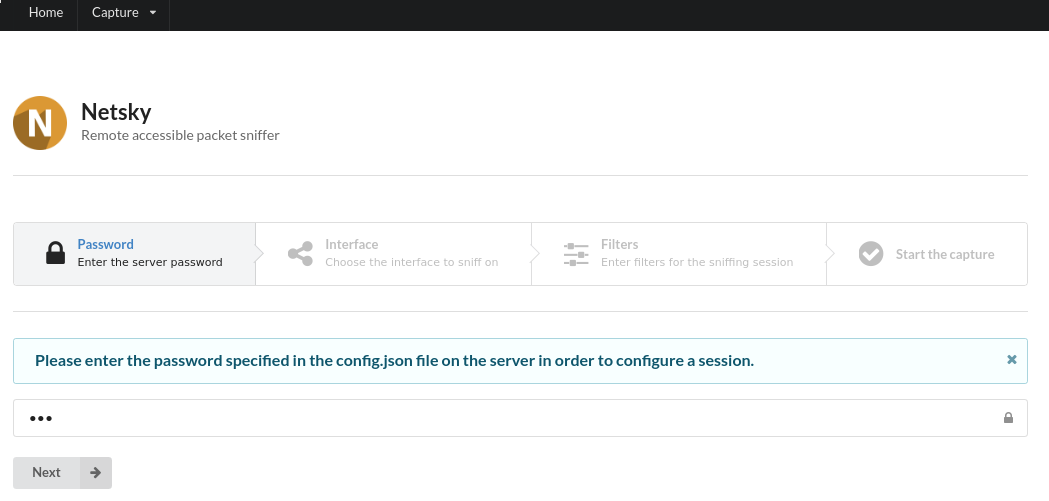
\includegraphics[width=\textwidth]{figures/screenshots/password.png}
  \caption{Въвеждане на парола за сесията.}
  \label{screenshots_password_fig}
\end{figure}

\subsection{Избор на мрежови интерфейс}

На мрежовия администратор се предоставя списък от имена на интерфейси, както и
адресите на тези, които имат такива: IP адрес, мрежова маска и т.н. За избор на
интерфейс е достатъчно да се започне въвеждането на името на интерфейса, след
това от падащото меню се избира чрез мишката или Enter. След избора на интерфейс,
\texttt{Next} бутона отвежда към следващата стъпка ---
въвеждането на филтриращ израз.

\begin{figure}[h!]
  \centering
  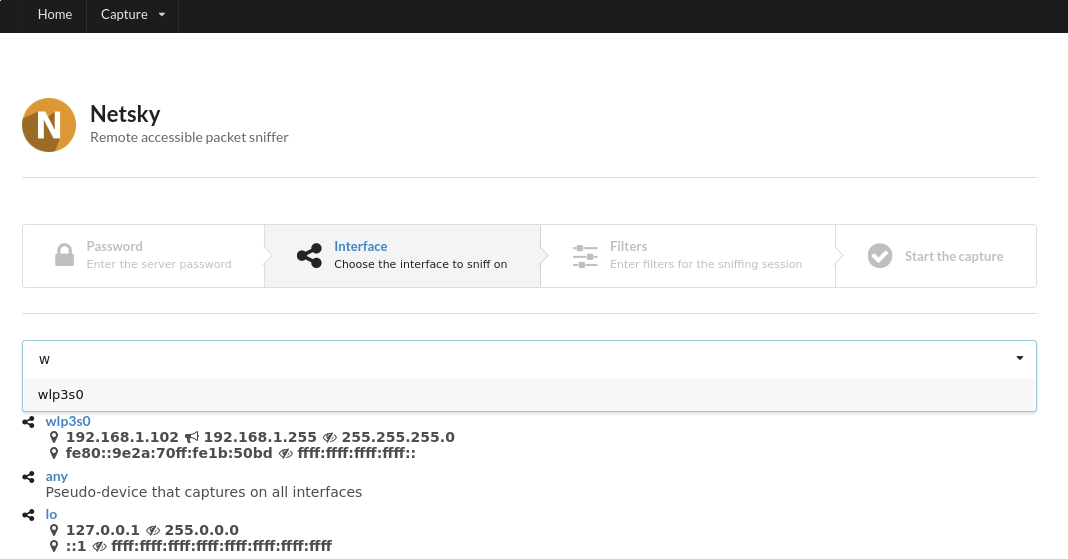
\includegraphics[width=\textwidth]{figures/screenshots/interface.png}
  \caption{Избор на физически интерфейс.}
  \label{screenshots_interface_fig}
\end{figure}

\subsection{Въвеждане на филтриращ израз}

Мрежовия администратор може да въведе филтър, който да е валиден за цялата сесия
на анализ. Например, филтърът \texttt{ip} прихваща само IP трафик. Съществуват
по-прости\footnote{\url{http://alumni.cs.ucr.edu/~marios/ethereal-tcpdump.pdf}}
филтри,
но и
комплексни\footnote{\url{https://www.wains.be/pub/networking/tcpdump_advanced_filters.txt}}
такива, с които може да се филтрира на ниво битове.

\begin{figure}[h!]
  \centering
  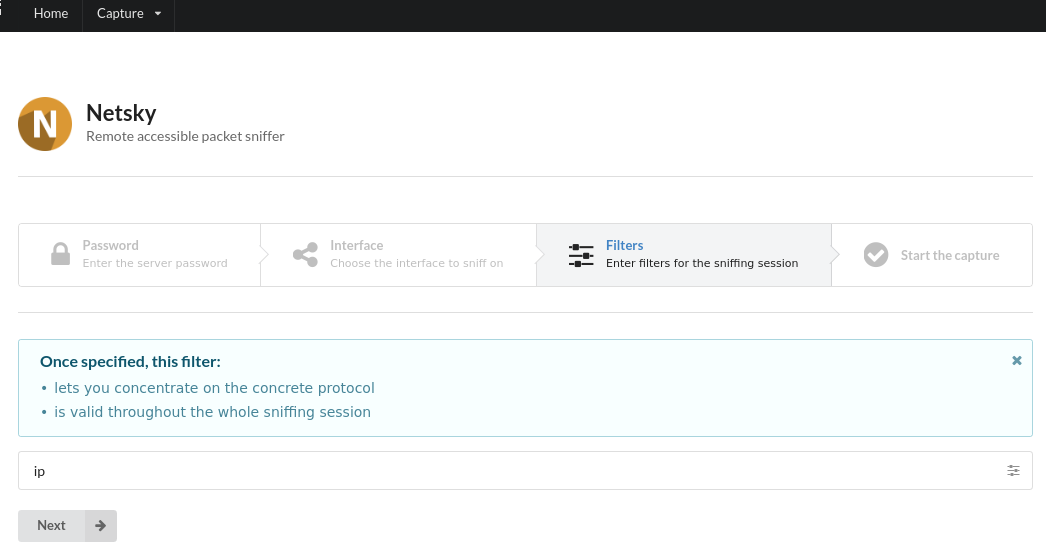
\includegraphics[width=\textwidth]{figures/screenshots/filter.png}
  \caption{Въвеждане на филтриращ израз.}
  \label{screenshots_filter_fig}
\end{figure}

Важно е да се отбележи, че с
оглед характера на анализатора, а именно поддръжащ отдалечен анализ, е почти
задължително анализиращия да въведе неговият публичен IP адрес като ненужен за
анализ. Това може да стане с простия филтър:

\begin{lstlisting}[caption=Филтър изолиращ адреса на
  отдалечения клиент от прихващаните пакети]
  host not <remote client IP>
\end{lstlisting}

\subsection{Стартиране на сесия}

След настройването на необходимите параметри на сесията, на мрежовия
администратор се представя екран на кратък обзор на конфигурираните параметри.
След натискането на \texttt{Start} бутона, сесията започва.

\begin{figure}[h!]
  \centering
  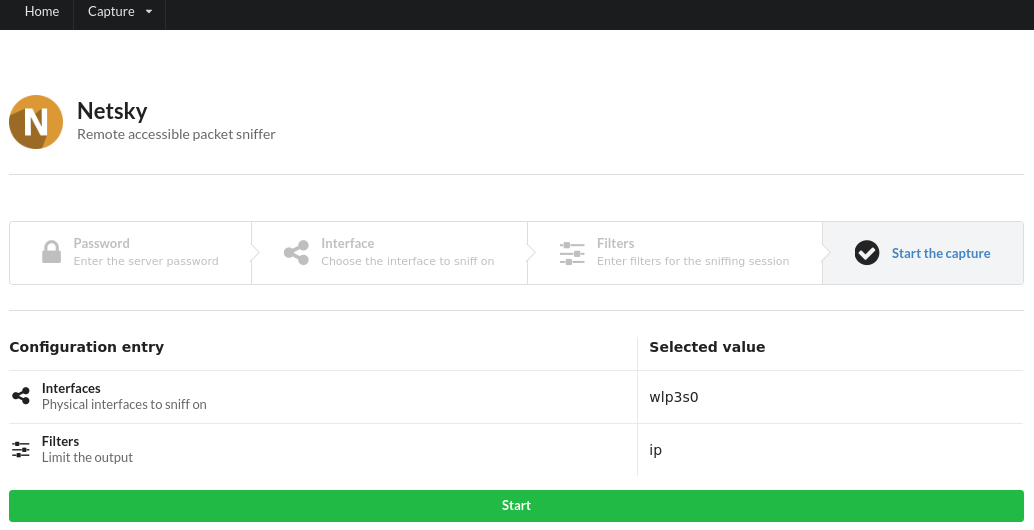
\includegraphics[width=\textwidth]{figures/screenshots/start.png}
  \caption{Стартиране на сесия.}
  \label{screenshots_start_fig}
\end{figure}

\subsection{Екран на сесия}

\begin{figure}[h!]
  \centering
  \includegraphics[width=\textwidth]{figures/screenshots/capture.png}
  \caption{Екран на сесия.}
  \label{capture_fig}
\end{figure}

В най-горната част на прозореца, представен на \autoref{capture_fig}, се представя списъка с пакети чрез обобщена
информация за пакета: логически и физически адрес на получателя, номерата на
портовете за съответните връзки. При натискане върху някой от пакетите, се
показват два допълнителни панела: детайлите на пакета и съдържанието на
полезната му информация.
За по-детайлен преглед на някое от свойствата на пакета се натиска конкретния
правоъгълник, който се мащабира. За демащабиране се натиска най-левия
правоъгълник, който връща изгледа към първоначалната цялостна структура на
кадъра.

Полето за филтриране поддържа филтрация на вече прихванататите пакети. То
поддържа JSQL
изрази\footnote{\url{https://github.com/deitch/searchjs/blob/master/README.md}}.
На практика може да се филтрира по всяко
едно поле, дори и то да е флаг, като то се достигне чрез наслагване на
свойствата на кадъра. Пример за по-прост филтър, базиращ се единствено на
обобщените свойства на пакета е:

\begin{lstlisting}[caption={Филтър, извеждащ само пакети с
  IP адрес на подателя \texttt{77.70.13.64}}]
  {"network.src": "77.70.13.64"}
\end{lstlisting}

С бутона \texttt{Apply filter} въведения филтър се
прилага, с \texttt{Clear filter} бутона се изчиства приложен филтър и списъка на
прихванати пакети се нулира към оригиналния. \texttt{Stop} бутона спира сесията
на анализ.

\subsection{Екран на абониране към вече съществуваща сесия}

В случай, че има вече инициирана сесия на анализ, новодостъпилия приложението
администратор бива пренасочен към екран на абониране за съществуващата сесия.

\begin{figure}[h!]
  \centering
  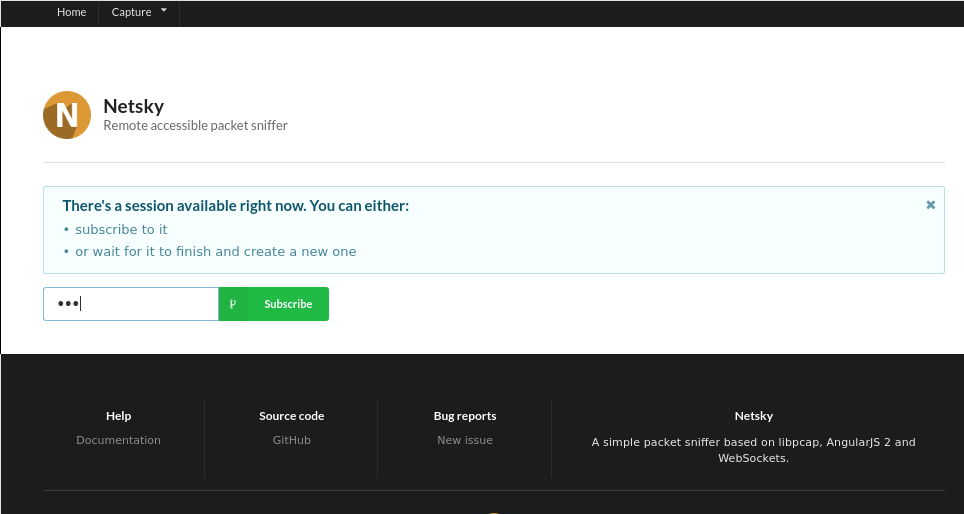
\includegraphics[width=\textwidth]{figures/screenshots/session-subscription.png}
  \caption{Екран на абониране към вече съществуваща сесия.}
  \label{capture_fig}
\end{figure}

В полето се въвежда паролата на сесията, след което се натиска
\texttt{Subscribe} бутона и администратора бива пренасочен към вече описания
екран на сесията.

\chapter{Заключение}

Представената дипломна работа реализира прост мрежов анализатор с възможност
за отдалечен преглед на анализа от няколко мрежови администратори.
Въпреки че не се стреми да осъществи анализ на голямо множество протоколи,
текущата имплементация предлага принципен модел на реализация, който се
цели да направи добавянето на такива лесно чрез прилагане на вече доказани
добри практики в обектно-ориентирания дизайн. Текущата имплементация включва
в себе си използването на широка гама технологии: от библиотеки на ниско ниво (libpcap),
през вече установени езици, поддържащи механизми за абстракция (C++11),
и модерни решения в лицето на Angular 2 и TypeScript.

В бъдеще, приложението би могло да имплементира следните функционалности:

\begin{itemize}
  \item
  да се добавят по-голямо количество поддържани протоколи
\item
  да се имплементира статистика на дистрибуцията на анализирани пакети,
  например карта на горещите точки (heatmap) за адресите на получателите, за
  да се види визуално географската дистрибуция на трафика
\item
  да се иплементира изваждане на текущия анализ във файлове в pcap формата;
  впоследствие те могат да се използват като входни данни на алгоритми за
  машинно самообучение и др. с цел допълнителен анализ: например, разбиране
  дали даден пакет е зловреден
\item
  да се интегрира анализатора със защитна стена или подобен механизъм
\end{itemize}

\bibliographystyle{abbrvnat}
\bibliography{literature/library}

\listoffigures

\newpage
\begin{flushleft}
\begin{Large}
\emph{\bf Списък на съкращения}\\
\end{Large}
\end{flushleft}
\begin{spacing}{1.241}
\vspace{10mm}
\begin{minipage}{0.2\textwidth}
\begin{flushleft} \normalsize
GUI\\
PDU\\
FDDI\\
ARP\\
RARP\\
DHCP\\
IP\\
ICMP\\
TCP\\
UDP\\
HTTP\\
FTP\\
SSH\\
DNS\\
SVG\\
GPL\\
RFC\\
SDK\\
API\\
\end{flushleft}
\end{minipage}
~
\begin{minipage}{0.5\textwidth}
\begin{flushleft} \normalsize
Graphical User Interface\\
Protocol Data Unit\\
Fiber Distributed Data Interface\\
Address Resolution Protocol\\
Reverse Address Resolution Protocol\\
Dynamic Host Configuration Protocol\\
Internet Protocol\\
Internet Control Message Protocol\\
Transmission Control Protocol\\
User Datagram Protocol\\
Hypertext Transfer Protocol\\
File Transfer Protocol\\
Secure Shell\\
Domain Name System\\
Scalable Vector Graphics\\
GNU General Public License\\
Request for Comments\\
Software Development Kit\\
Application Programming Interface\\
\end{flushleft}
\end{minipage}\\[4cm]
\end{spacing}
\vfill
\end{document}
